\documentclass[12pt]{article}

\usepackage[]{graphicx}
\usepackage[]{color}
\usepackage{alltt}
% packages not included in template
\usepackage{amsmath}
\usepackage{placeins}
\usepackage{amssymb}
\usepackage{subcaption}
\usepackage{booktabs}


\newcommand{\mytitle}{MC‑Dropout and SWAG for Uncertainty Estimation in Neural Networks}
\newcommand{\myname}{Martin Kandlinger}
\newcommand{\mysupervisor}{Dr. Ludwig Bothmann}

\usepackage[a4paper, width = 160mm, top = 35mm, bottom = 30mm, 
bindingoffset = 0mm]{geometry}
\usepackage[utf8]{inputenc}
\usepackage{ragged2e}
\usepackage{xcolor}
\usepackage[round, comma]{natbib}
\usepackage{fancyhdr}
\newcommand{\changefont}{%
    \fontsize{8}{11}\selectfont
}
\usepackage{hyperref}
\hypersetup{
  colorlinks = true,
  linkcolor = black,
  urlcolor = black,
  citecolor = black}
\pagestyle{fancy}
\fancyhead{}
\fancyhead[R]{\changefont{\mytitle}}
\fancyfoot{}
\fancyfoot[R]{\thepage}
\setlength{\headheight}{14.5pt}
\setlength{\parindent}{0pt}
\interfootnotelinepenalty = 10000

% ------------------------------------------------------------------------------
% MAIN -------------------------------------------------------------------------
% ------------------------------------------------------------------------------
\IfFileExists{upquote.sty}{\usepackage{upquote}}{}
\begin{document}

% FRONT PAGE -------------------------------------------------------------------
 
\begin{titlepage}
\begin{center}
    
\LARGE
Bachelor's Seminar
    
\vspace{0.5cm}
      
\rule{\textwidth}{1.5pt}
\LARGE
\textbf{\mytitle}
\rule{\textwidth}{1.5pt}
   
\vspace{0.5cm}
      
\large
Department of Statistics \\
Ludwig-Maximilians-Universität München 

\vfill

\Large
\textbf{\myname}

\vfill

\large
Munich, Juli 6\textsuperscript{th}, 2025
      
\vfill


\includegraphics[width = 0.4\textwidth]{sigillum.png}

\vfill

\normalsize
Submitted in partial fulfillment of the requirements for the degree of B. Sc.
\\
Supervised by \mysupervisor

\end{center}
\end{titlepage}

% CONTENTS ---------------------------------------------------------------------

\pagenumbering{Roman}
\newpage

\begin{abstract}
Estimating uncertainty in deep neural networks is essential for reliable decision making, especially in
high stakes applications. This work examines two practical approximation methods, Monte Carlo Dropout
(MC-Dropout) and Stochastic Weight Averaging Gaussian (SWAG), for their effectiveness in uncertainty
quantification. A unified evaluation framework assesses both methods on synthetic datasets, where
uncertainty behavior is controllable and a real-world benchmark, the Boston Housing dataset. Metrics
include calibration quality, predictive accuracy, and robustness under distribution shift. Results
indicate that MC-Dropout provides a computationally efficient uncertainty estimation, whereas SWAG yields
richer posterior approximations and improved calibration. Practical recommendations are provided to guide
method selection according to specific application requirements.

% for calibration quality NLL, PICP
% for predictive accuracy RMSE
\end{abstract}

\newpage
\tableofcontents

%%%% if you would want to include material overview
%%%% use one of the following in addition
% \newpage
% \listoffigures
% \newpage
% \listoftables
\newpage

% ------------------------------------------------------------------------------
% CHAPTERS ---------------------------------------------------------------------
% ------------------------------------------------------------------------------

\pagenumbering{arabic}
    
\section{Introduction}
\label{intro}

Deep neural networks (DNNs) have achieved remarkable success across domains such as computer vision,
natural language processing, and healthcare. When deploying such models in critical applications 
regarding safety, such as autonomous driving, medical diagnosis, or financial risk assessment,
quantifying model uncertainty becomes essential. Overconfident predictions on noisy or
out-of-distribution inputs can lead to disastrous outcomes and undermine
trust in machine learning systems \citep{pereira2020challenges, valentin2024certification}.

\vspace{0.15cm}
In predictive modeling, uncertainty arises from two main sources: aleatoric uncertainty,
which is inherent noise in the data (e.g., sensor noise or label ambiguity) and epistemic uncertainty,
which stems from limited data, incomplete knowledge, or insufficient model capacity. Unlike aleatoric
uncertainty, epistemic uncertainty can be reduced by collecting more observations or employing a more
appropriate model architecture that better captures the underlying function
\citep{hullermeier2021aleatoric}. This work focuses on the quantification of epistemic uncertainty,
as it signals when models operate beyond their knowledge boundaries.

\vspace{0.15cm}
We evaluate two practical approximation methods, Monte Carlo Dropout (MC-Dropout) and Stochastic Weight
Averaging Gaussian (SWAG). MC‑Dropout offers a lightweight approach by retaining dropout during inference,
effectively simulating Bayesian sampling through multiple stochastic forward passes without altering the
models architecture \citep{gal2016mcdropout}. SWAG constructs a Gaussian posterior over the model weights
by capturing stochastic gradient descent (SGD) trajectory moments during training, offering richer
uncertainty representations with improved robustness to distribution shifts \citep{maddox2019swag}.

\vspace{0.15cm}
After presenting these methods, their performance will be compared within a unified experimental framework.
Both MC‑Dropout and SWAG are applied to synthetic datasets, where true uncertainty is known,
and also to real‑world data (the boston housing dataset with ethical preprocessing). The evaluation metrics
include predictive accuracy (RMSE), calibration quality (NLL, PICP), and out-of-distribution reliability.

\vspace{0.15cm}
The work is structured as follows: Section \ref{related_work} reviews prior work on uncertainty
quantification methods and Bayesian neural models,
Section \ref{methodology} details the MC‑Dropout and SWAG approaches,
but also explains the underlying mechanisms and prior knowledge needed to understand them,
Section \ref{experiments} presents comparative evaluations,
Section \ref{discussion} analyzes trade-offs and future extensions and
Section \ref{conclusion} summarizes key findings and their implications.

\newpage

\section{Related Work}
\label{related_work}

A diverse set of techniques has been proposed for quantifying uncertainty in neural networks, which can
broadly be categorized into variational approaches, ensemble methods and approximate inference techniques.

\paragraph{Variational Approaches}
Monte Carlo Dropout (MC-Dropout), introduced by \citet{gal2016mcdropout}, implements variational
inference by retaining dropout at test time to obtain uncertainty estimates. While computationally
efficient, subsequent research has identified limitations. MC-Dropout can underestimate uncertainty,
particularly in regions with little to no data \citep{osband2016}, which aligns with our observations of
undercoverage and overconfidence in Section \ref{exp:real-world_data}. \citet{verdoja2021behaviormcdropout}
demonstrate that model architecture, training and tuning choices heavily influence the estimated
uncertainty. Furthermore, \citet{sicking2020characteristicsmcdropout} observe that MC-Dropout may produce
non-Gaussian uncertainty distributions in wide networks.

Another noteworthy approach is Bayes by Backprop \citep{blundell2015bayesbybackprop}. This method
places a distribution (typically Gaussian) over model weights, learned via variational inference.
The resulting weight uncertainty can then be used to generate predictive uncertainty estimates
through weight sampling.

\paragraph{Ensemble Methods}
Deep Ensembles \citep{lakshminarayanan2017preduncw/deepensembles} combine predictions from multiple
independently trained models and consistently outperform MC-Dropout, especially under dataset shifts,
as shown by \citet{fort2020deepensembles}. They require high computational and memory costs, which makes
them less practical for large-scale applications.

Stochastic Weight Averaging Gaussian (SWAG), introduced by \citet{maddox2019swag}, constructs a Gaussian
posterior over weights based on Stochastic Gradient Descent (SGD) trajectory statistics. As validated in
our experiments (Section \ref{exp:real-world_data}), SWAG demonstrates improved calibration and robustness
compared to MC-Dropout while maintaining reasonable computational overhead. The Extension MultiSWAG
\citep{onal2024multiswag} bridges the gap between SWAG and full ensembles.

\paragraph{Approximate Inference}
Methods like Laplace approximations, expectation propagation perform local Gaussian posterior approximation
around a maximum a posteriori (MAP) estimation. These methods yield competitiveperformance in both
efficiency and uncertainty quality \citep[see, e.g.,][]{ritter2018kfaclaplace}. Linearized Laplace
\citep{antoran2022linearizedlaplace}, and more efficient variants such as Laplace Redux
\citep{daxberger2022laplaceredux} offer scalable posterior estimation with good calibration and
performance. These techniques offer a middle ground between simplicity and robustness.

\vspace{0.4cm}
This work focuses on MC-Dropout and SWAG, which cover both ends of the trade-off spectrum discussed in
prior work. MC-Dropout for its ease-of-use and efficiency, and SWAG for its richer posterior structure
and empirical strength.


\newpage

\section{Methodology}
\label{methodology}

This section presents the theoretical foundations and detailed mechanics necessary to understand
the methods used in Section \ref{experiments}.

\subsection{Bayesian Neural Networks}
\label{methodology:bnns}
Bayesian inference allows updating prior beliefs using previously unseen data via Bayes' theorem:

\begin{equation}
P(\theta \mid \mathcal{D}) = \frac{P(\mathcal{D} \mid \theta) P(\theta)}{P(\mathcal{D})} 
\quad \text{where} \quad 
P(\mathcal{D}) = \int P(\mathcal{D} \mid \theta') P(\theta')  d\theta'
\label{eq:bayes}
\end{equation}

Here, $P(\theta)$ is the prior distribution over parameters, $P(\mathcal{D} \mid \theta)$ is the
likelihood (encoding aleatoric uncertainty), and $P(\theta \mid \mathcal{D})$ is the posterior
(capturing epistemic uncertainty) \citep{Jospin2022bnns}.
This formalism enables quantification of both uncertainty types.

\vspace{0.15cm}
Before introducing Bayesian neural networks, we briefly recall the fundamentals of standard neural
networks. Artificial neural networks (NNs) are inspired by biological brains, they consist of layered
interconnected neurons. Each neuron computes a weighted sum of inputs $x_i$ plus a bias $b$
and applies a nonlinear activation function $g(\cdot)$:

\[
z = \sum_{i} w_i x_i + b, \quad \text{output} = g(z)
\]

In a deep neural network, neurons are organized in multiple layers. During training, the network adjusts
its parameters (weights $\mathbf{W}$ and biases $\mathbf{b}$) via backpropagation and gradient
descent to minimize a loss function on training data \citep{Haykin2009, López2022anns&dl}.
These learned parameters are treated as fixed point estimates at test time, and the network produces a
single prediction without expressing uncertainty. So while NNs are powerful in pattern recognition,
they lack a mechanism to quantify confidence in their predictions.

\vspace{0.15cm}
Bayesian Neural Networks (BNNs) address this limitation by treating weights $\mathbf{W}$ as random 
variables with specified prior distributions. Given training data $\mathcal{D} = \{(x_i, y_i)\}$,
Bayes' theorem yields the posterior distribution:
% Bayesian Neural Networks (BNNs) are stochastic neural networks trained using Bayesian inference \citep[see, e.g.,][]{Jospin2022bnns}.

\begin{equation}
p(\mathbf{W} \mid \mathcal{D}) = \frac{p(\mathcal{D} \mid \mathbf{W})  p(\mathbf{W})}{p(\mathcal{D})}
\label{eq:posterior}
\end{equation}

Predictions incorporate uncertainty through marginalization over the posterior:

\begin{equation}
p(y^* \mid x^*, \mathcal{D}) = \int p(y^* \mid x^*, \mathbf{W})  p(\mathbf{W} \mid \mathcal{D})  d\mathbf{W}
\label{eq:predictive}
\end{equation}

Unlike deterministic NNs, BNNs output predictive distributions where variance reflects model confidence.
Narrow distributions indicate high certainty, while broad distributions reveal epistemic uncertainty,
especially in regions with limited data \citep{Jospin2022bnns}.

Training a BNN involves specifying a prior $p(\mathbf{W})$ and computing the posterior $p(\mathbf{W}
\mid \mathcal{D})$. However, computing the exact posterior is not feasible for modern deep networks
because it requires calculating $p(\mathcal{D})$ in Eq.~\eqref{eq:posterior}, which is the integral
shown in Eq.~\eqref{eq:bayes}. It integrates over the weight space, for modern NNs with millions of
weights, this integral requires massive amounts of computing power. Furthermore, predictions require
solving yet another high-dimensional integral (Eq.~\eqref{eq:predictive}) over the same parameter
space. Consequently, approximate inference methods are essential, as discussed in subsequent sections.


\subsection{Dropout Regularization}
\label{methodology:dropout}
Dropout, introduced by \citet{srivastava2014dropout}, is a regularization technique for neural networks.
During training, dropout temporarily removes a random subset of neurons by multiplying their activations
with independent Bernoulli-distributed variables:

\[
r_j^{(l)} \sim \operatorname{Bernoulli}(p), 
\quad 
\tilde{\mathbf{y}}^{(l)} = \mathbf{r}^{(l)} \odot \mathbf{y}^{(l)}
\]

where $p$ is the retention probability (dropout rate = $1-p$) and $\mathbf{r}^{(l)}$ is a binary mask vector for layer $l$.

A key motivation for dropout is to prevent co-adaptation. In standard neural networks,
neurons may develop complex interdependencies that cause them to function only in specific combinations.
This means if one neuron fails (e.g., due to a noisy input), the entire model may break down,
leading to poor generalization and overfitting \citep{hinton2012}.
Dropout improves robustness by forcing neurons to
learn useful features independently.

This process effectively trains an ensemble of exponentially many "thinned" subnetworks that share
weights, which prevents complex co-adaptation of features and improves generalization \citep{srivastava2014dropout}.

\begin{figure}[htbp]
    \centering
    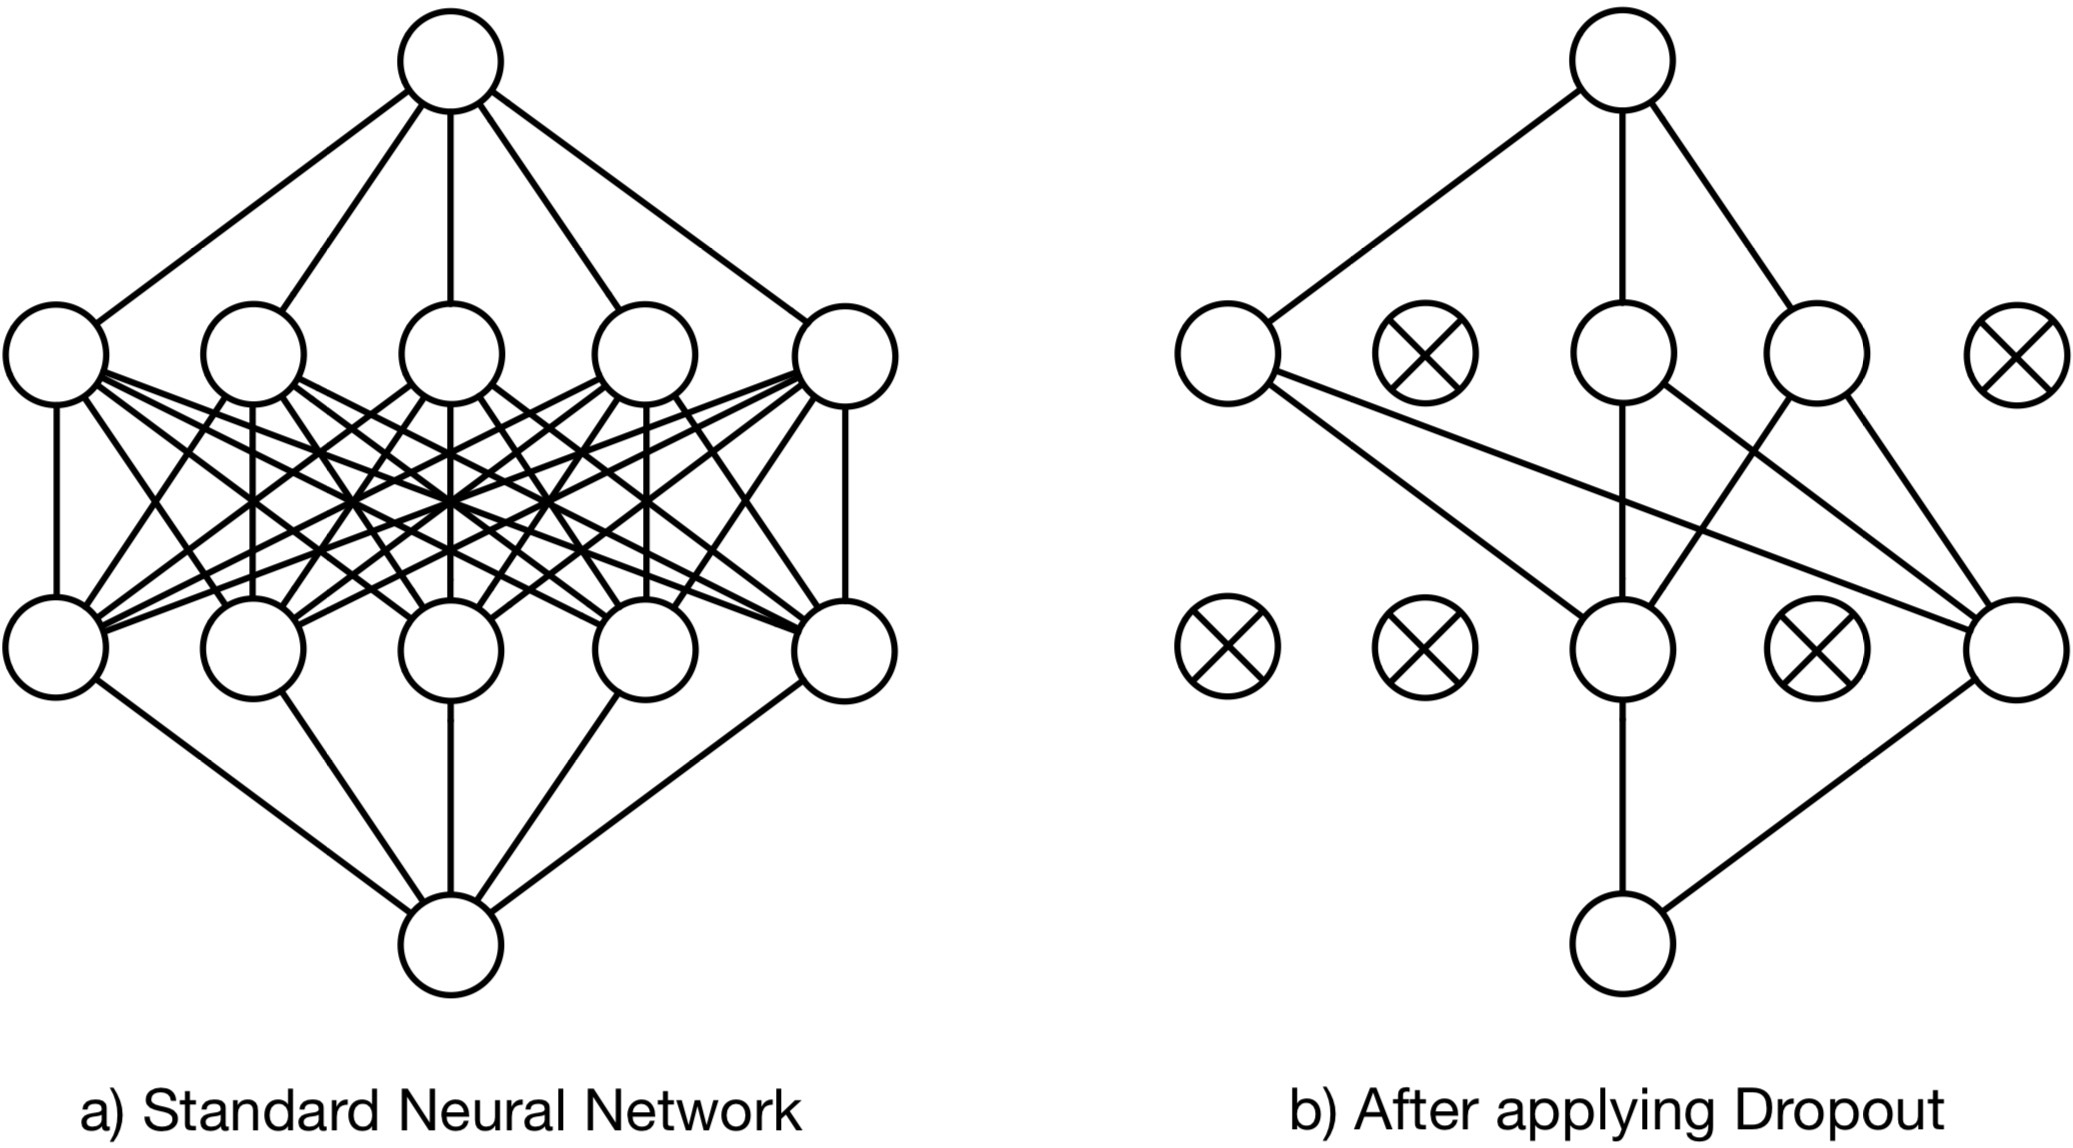
\includegraphics[width=0.65\linewidth]{figures/fig_dropout.png}
    \caption{Visualization of the dropout mechanism: (a) Standard neural network with two hidden layers; (b) Thinned network after applying dropout masks. Crossed neurons are temporarily deactivated during training.\\
    This figure was manually reillustrated with minor adjustments, the original version was published by \citet{srivastava2014dropout}}
    \label{fig:dropout-srivastava}
\end{figure}

At test time, averaging across all possible thinned subnetworks is infeasible due to the exponential
growth of possible configurations with increasing network size. Instead, dropout is disabled, resulting
in a single network. Each of the network's weights is scaled by $p$, which approximates the geometric
mean of predictions from all subnetworks without the heavy computation needed for explicit averaging.

\vspace{0.15cm}
Unlike Monte Carlo Dropout, standard dropout functions purely as a regularizer, which means it
improves generalization and reduces overfitting but doesn't provide uncertainty estimates
\citep{srivastava2014dropout}.


\subsection{Monte Carlo Dropout}
\label{methodology:mcd}
\citet{gal2016mcdropout} introduced Monte Carlo dropout (MC-Dropout) as an efficient method to estimate
uncertainty in neural networks. Unlike classic dropout, MC-Dropout keeps dropout active during testing.
It performs multiple stochastic forward passes through the network, each with different randomly
activated neurons, effectively sampling predictions $\{f^{\hat{\mathbf{W}}_t}(x^*)\}_{t=1}^T$ from $T$
thinned subnetworks. Each subnetwork's weights $\hat{\mathbf{W}}_t$ can be thought of as a sample from
the posterior $p(\mathbf{W} \mid \mathcal{D})$ and each prediction $f^{\hat{\mathbf{W}}_t}(x^*)$ as a
sample from the predictive distribution $p(y^* \mid x^*, \mathcal{D})$. The predictive distribution
quantifies the uncertainty about the models response for a new observation $x^*$ given the observed data.

The collection of these predictions forms a distribution where the mean approximates the expected
output and the variance quantifies epistemic uncertainty. Tightly clustered predictions indicate
high confidence, while dispersed predictions reveal model uncertainty.

\begin{figure}[htbp]
    \centering
    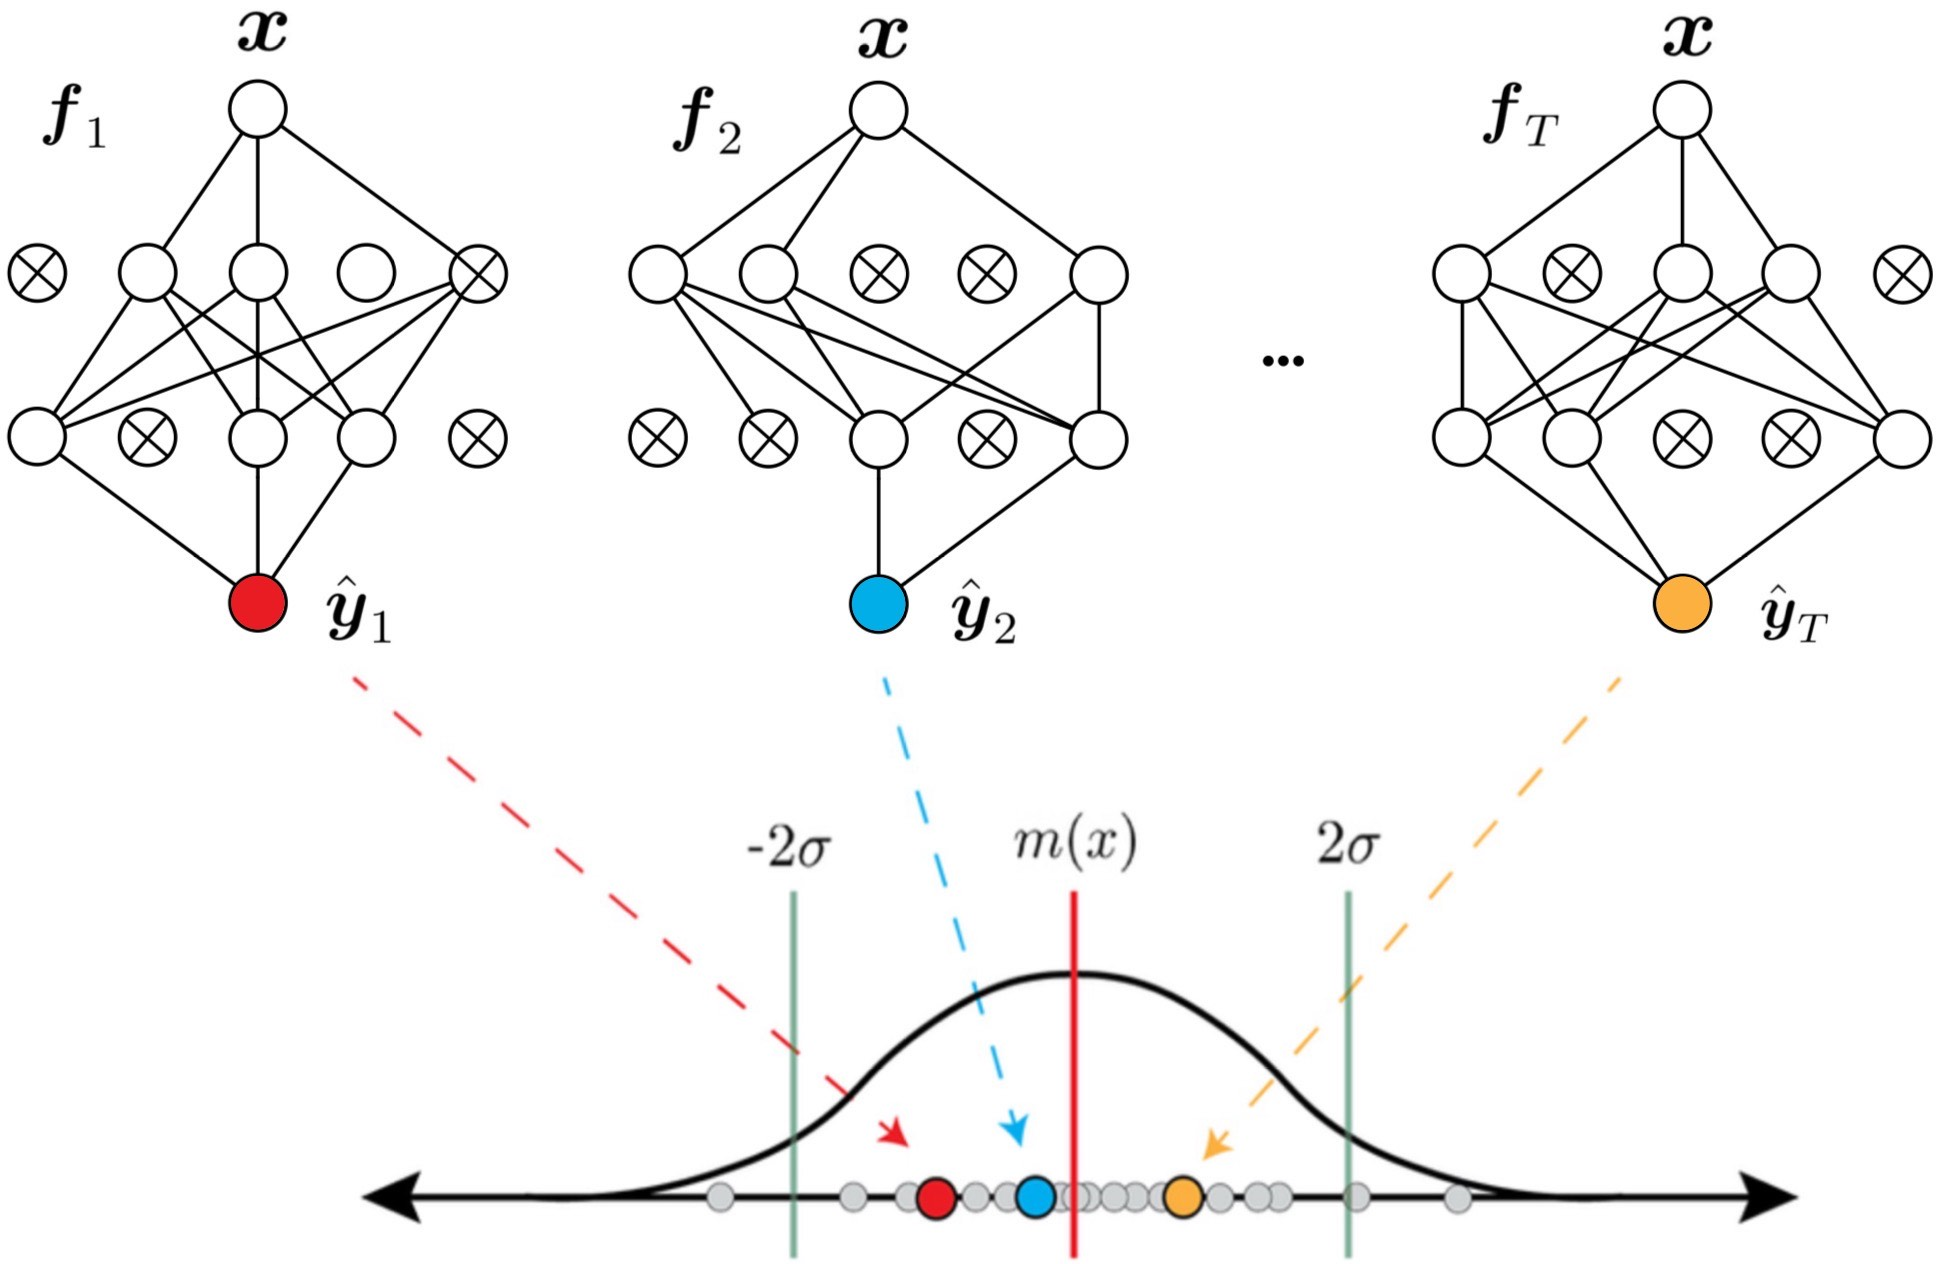
\includegraphics[width=0.65\linewidth]{figures/fig_mcd.png}
    \caption{MC-Dropouts predictive distribution. Colored and grey dots represent predictions from different thinned networks, crossed neurons are deactivated.\\This figure was manually reillustrated with minor adjustments, the original version was published by \citet{Katwyk2023}}
    \label{fig:mc-dropout2}
\end{figure}

MC-Dropout provides a Bayesian approximation without formal Bayesian neural networks.
By interpreting dropout as variational inference, it mimics posterior sampling through the predictive
distribution of subnetworks \citep{gal2016mcdropout}.

\vspace{0.15cm}
\textbf{Advantages:} MC-Dropout introduces minimal computational overhead since it requires only one
trained model and uses the same computational graph with dropout enabled during inference. It scales
efficiently, providing reasonable uncertainty estimates with significantly lower cost than full
ensembling. Implementation is straightforward in popular frameworks like PyTorch and TensorFlow.

\vspace{0.15cm}
\textbf{Limitations:} The method tends to underestimate uncertainty in data-sparse regions and may not
concentrate appropriately as the amount of data increases \citep{osband2016}.
The estimated uncertainty is sensitive to changes in hyperparameters (e.g. retention probability $p$)
\citep{verdoja2021behaviormcdropout}.
As a variational method, MC-Dropout primarily explores uncertainty around a single point (mode) in the
posterior space, potentially underestimating the true posteriors variance. This makes sense because the
diversity among subnetworks is low, since all of them are dropout versions of the main network.
In contrast, deep ensembles with independently trained models capture multiple modes, offering
greater predictive diversity and robustness to distribution shifts \citep{fort2020deepensembles}.

\vspace{0.15cm}
Despite its limitations, MC-Dropout remains a popular baseline for practical uncertainty quantification
due to its simplicity, low computational cost (especially compared to ensemble techniques, as the model
is trained only once), and compatibility with other uncertainty estimation methods. It is particularly
advantageous when training resources are limited or when the true posterior distribution is expected to be simple.


\subsection{Stochastic Weight Averaging Gaussian}
\label{methodology:swag}
Stochastic Weight Averaging with Gaussian posterior approximation (SWAG) builds on Stochastic Weight
Averaging (SWA), a technique introduced by \citet{izmailov2019swa}. The core idea behind SWA is,
that after training a neural network normally, one restarts stochastic gradient descent (SGD) from that
trained state using a constant or cyclical learning rate to explore the weight space. The weights $w_i$
obtained after each iteration $i$ of the SGD algorithm are periodically saved and once the algorithm
finishes after $T$ or more iterations, the SWA mean (or SWA solution) is computed:

\[
\mathbf{w}_{\mathrm{SWA}} = \frac{1}{T}\sum_{i=1}^T \mathbf{w}_i
\]

\citet{izmailov2019swa} argue, that the SWA mean converges toward the center of a wide, flat region in
the loss surface, which leads to a more robust model and better generalization compared to the solution
that conventional SGD produces.

\vspace{0.15cm}
SWAG \citep{maddox2019swag} extends SWA by constructing a Gaussian posterior approximation from these
weight snapshots. It estimates not just the mean $\mathbf{w}_{\mathrm{SWA}}$, but also a covariance
matrix capturing parameter uncertainty. The covariance comprises two complementary components:

\begin{enumerate}
    \item \textbf{Diagonal covariance ($\Sigma_{\mathrm{diag}}$):} Computes per-parameter variance\\
    $\Sigma_{\mathrm{diag}} = \mathrm{diag}\left(\frac{1}{T-1}\sum_{i=1}^T (\mathbf{w}_i - \mathbf{w}_{\mathrm{SWA}})^2\right)$.\\
    This captures independent uncertainty estimates for individual weights.
          
    \item \textbf{Low-rank covariance ($\Sigma_{\mathrm{low\text{-}rank}}$):} Constructed from deviation
    vectors\\
    $\Sigma_{\mathrm{low\text{-}rank}} = \frac{1}{2(T-1)}\mathbf{D}\mathbf{D}^\top$  
    where $\mathbf{D} = [\mathbf{w}_1 - \mathbf{w}_{\mathrm{SWA}}, \dots, \mathbf{w}_T - \mathbf{w}_{\mathrm{SWA}}]$.\\
    This low-rank approximation captures dominant correlations between parameters.
\end{enumerate}

The combined covariance $\Sigma = \Sigma_{\mathrm{diag}} + \Sigma_{\mathrm{low\text{-}rank}}$ addresses
limitations of purely diagonal approximations, which often underestimate uncertainty by ignoring
parameter correlations \citep{maddox2019swag}. The full posterior approximation is:

\[
q_{\mathrm{SWAG}}(\mathbf{w}) = \mathcal{N}\left(\mathbf{w}_\mathrm{SWA}, \Sigma_\mathrm{diag} + \Sigma_\mathrm{low\text{-}rank}\right)
\]

At test time, SWAG samples weights $\mathbf{w}^{(s)} \sim q_{\mathrm{SWAG}}$ and computes predictions
$f^{\mathbf{w}^{(s)}}(x^*)$ for each sample. The resulting empirical distribution estimates the
predictive distribution $p(y^* \mid x^*, \mathcal{D})$, which as stated in Section \ref{methodology:mcd}
quantifies the uncertainty about the models response for a new observation given the observed data, its
mean approximates the expected output and its variance the epistemic uncertainty.

\vspace{0.15cm}
\textbf{Advantages:} By analyzing the SGD weight trajectories, SWAG captures posterior structure around
flat minima in the loss surface. While more computationally intensive than MC-Dropout, since it requires
extended training for weight exploration and covariance calculation, it remains significantly cheaper
than full ensembles because only one model is trained. \citet{maddox2019swag} demonstrate its superior
uncertainty calibration and robustness to distribution shifts compared to MC-Dropout and other
baselines, particularly on vision benchmarks like CIFAR and ImageNet.

\vspace{0.15cm}
\textbf{Limitations:} Although SWAG approximates uncertainty better than simpler methods, it still,
similar to MC-Dropout, represents a single mode of the posterior and does not learn true multimodal
structures \citep{onal2024multiswag}. Memory requirements increase with snapshot frequency due to
covariance storage, though remain manageable versus full ensembles. The quality of the uncertainty
estimation depends on the learning rate set for the exploration phase \citep{maddox2019swag}.

\vspace{0.15cm}
SWAG thus provides an efficient midpoint between simple variational methods and computationally
intensive approaches, offering structured uncertainty estimation with minimal training overhead beyond
standard SGD.
\newpage

\newpage

\section{Experiments}
\label{experiments}

This section applies the methods introduced in Section \ref{methodology} to both synthetic and
real‑world datasets and evaluates their capabilities in predictive accuracy, uncertainty calibration, and out-of-distribution (OOD) detection.

\subsection{Synthetic Dataset}
\label{exp:synthetic}
To evaluate MC-Dropout and SWAG for uncertainty quantification, experiments are conducted on a synthetic 
regression and binary classification task. Both tasks used a neural network with two fully-connected
hidden layers (32 neurons each with ReLU activations). For MC‑Dropout, dropout layers are added
after each hidden layer.

\paragraph{Regression Task}
A synthetic dataset is generated following:
\[
y = \sin(x) + 0.3\varepsilon, \quad \varepsilon \sim \mathcal{N}(0,1)
\]
Both models are trained on $x \in [-5, 5]$ and evaluated on $x \in [-8, 8]$.

\vspace{0.15cm}
As shown in Figure \ref{fig:regression}, both methods produce accurate mean predictions within the training region ($|x| \leq 5$), closely approximating $\sin(x)$. SWAG estimates thinner
uncertainty intervals than MC-Dropout, aligning with findings by \citet{maddox2019swag}.

Outside this region, the uncertainty bands increase as both methods detect OOD inputs. MC-Dropout
exhibits faster uncertainty growth, with uncertainty intervals widening more rapidly than SWAG beyond
$|x| > 5$. SWAG maintains tighter confidence bands while still showing some uncertainty expansion.

The sample points form vertical patterns ("pillars") in both cases. These result from 200 stochastic
predictions being sampled at each of the 100 equidistant test points along the x-axis. For MC-Dropout,
predictions come from different thinned subnetworks, while for SWAG they derive from weight samples
$\mathbf{w}^{(s)} \sim q_{\mathrm{SWAG}}$.

SWAG's samples follow a certain structure, where connecting e.g. the maximum prediction at each test
point will form a smooth curve. This is because these samples come from the same set of weights,
i.e. the same model. MC-Dropout's more irregular dispersion reflects the random neuron deactivations
from different dropout masks \citep{gal2016mcdropout}.

\vspace{0.15cm}
These observations align with theoretical expectations, MC-Dropout's sampling produces noisier but more
conservative uncertainty estimates \citep{gal2016mcdropout}, while SWAG's weight-space sampling provides
a geometrically structured uncertainty quantification. Both methods distinguish between in-domain
confidence and out-of-domain uncertainty.

\FloatBarrier

\begin{figure}[ht]
  \centering
  \begin{subfigure}{0.8\textwidth}
    \centering
    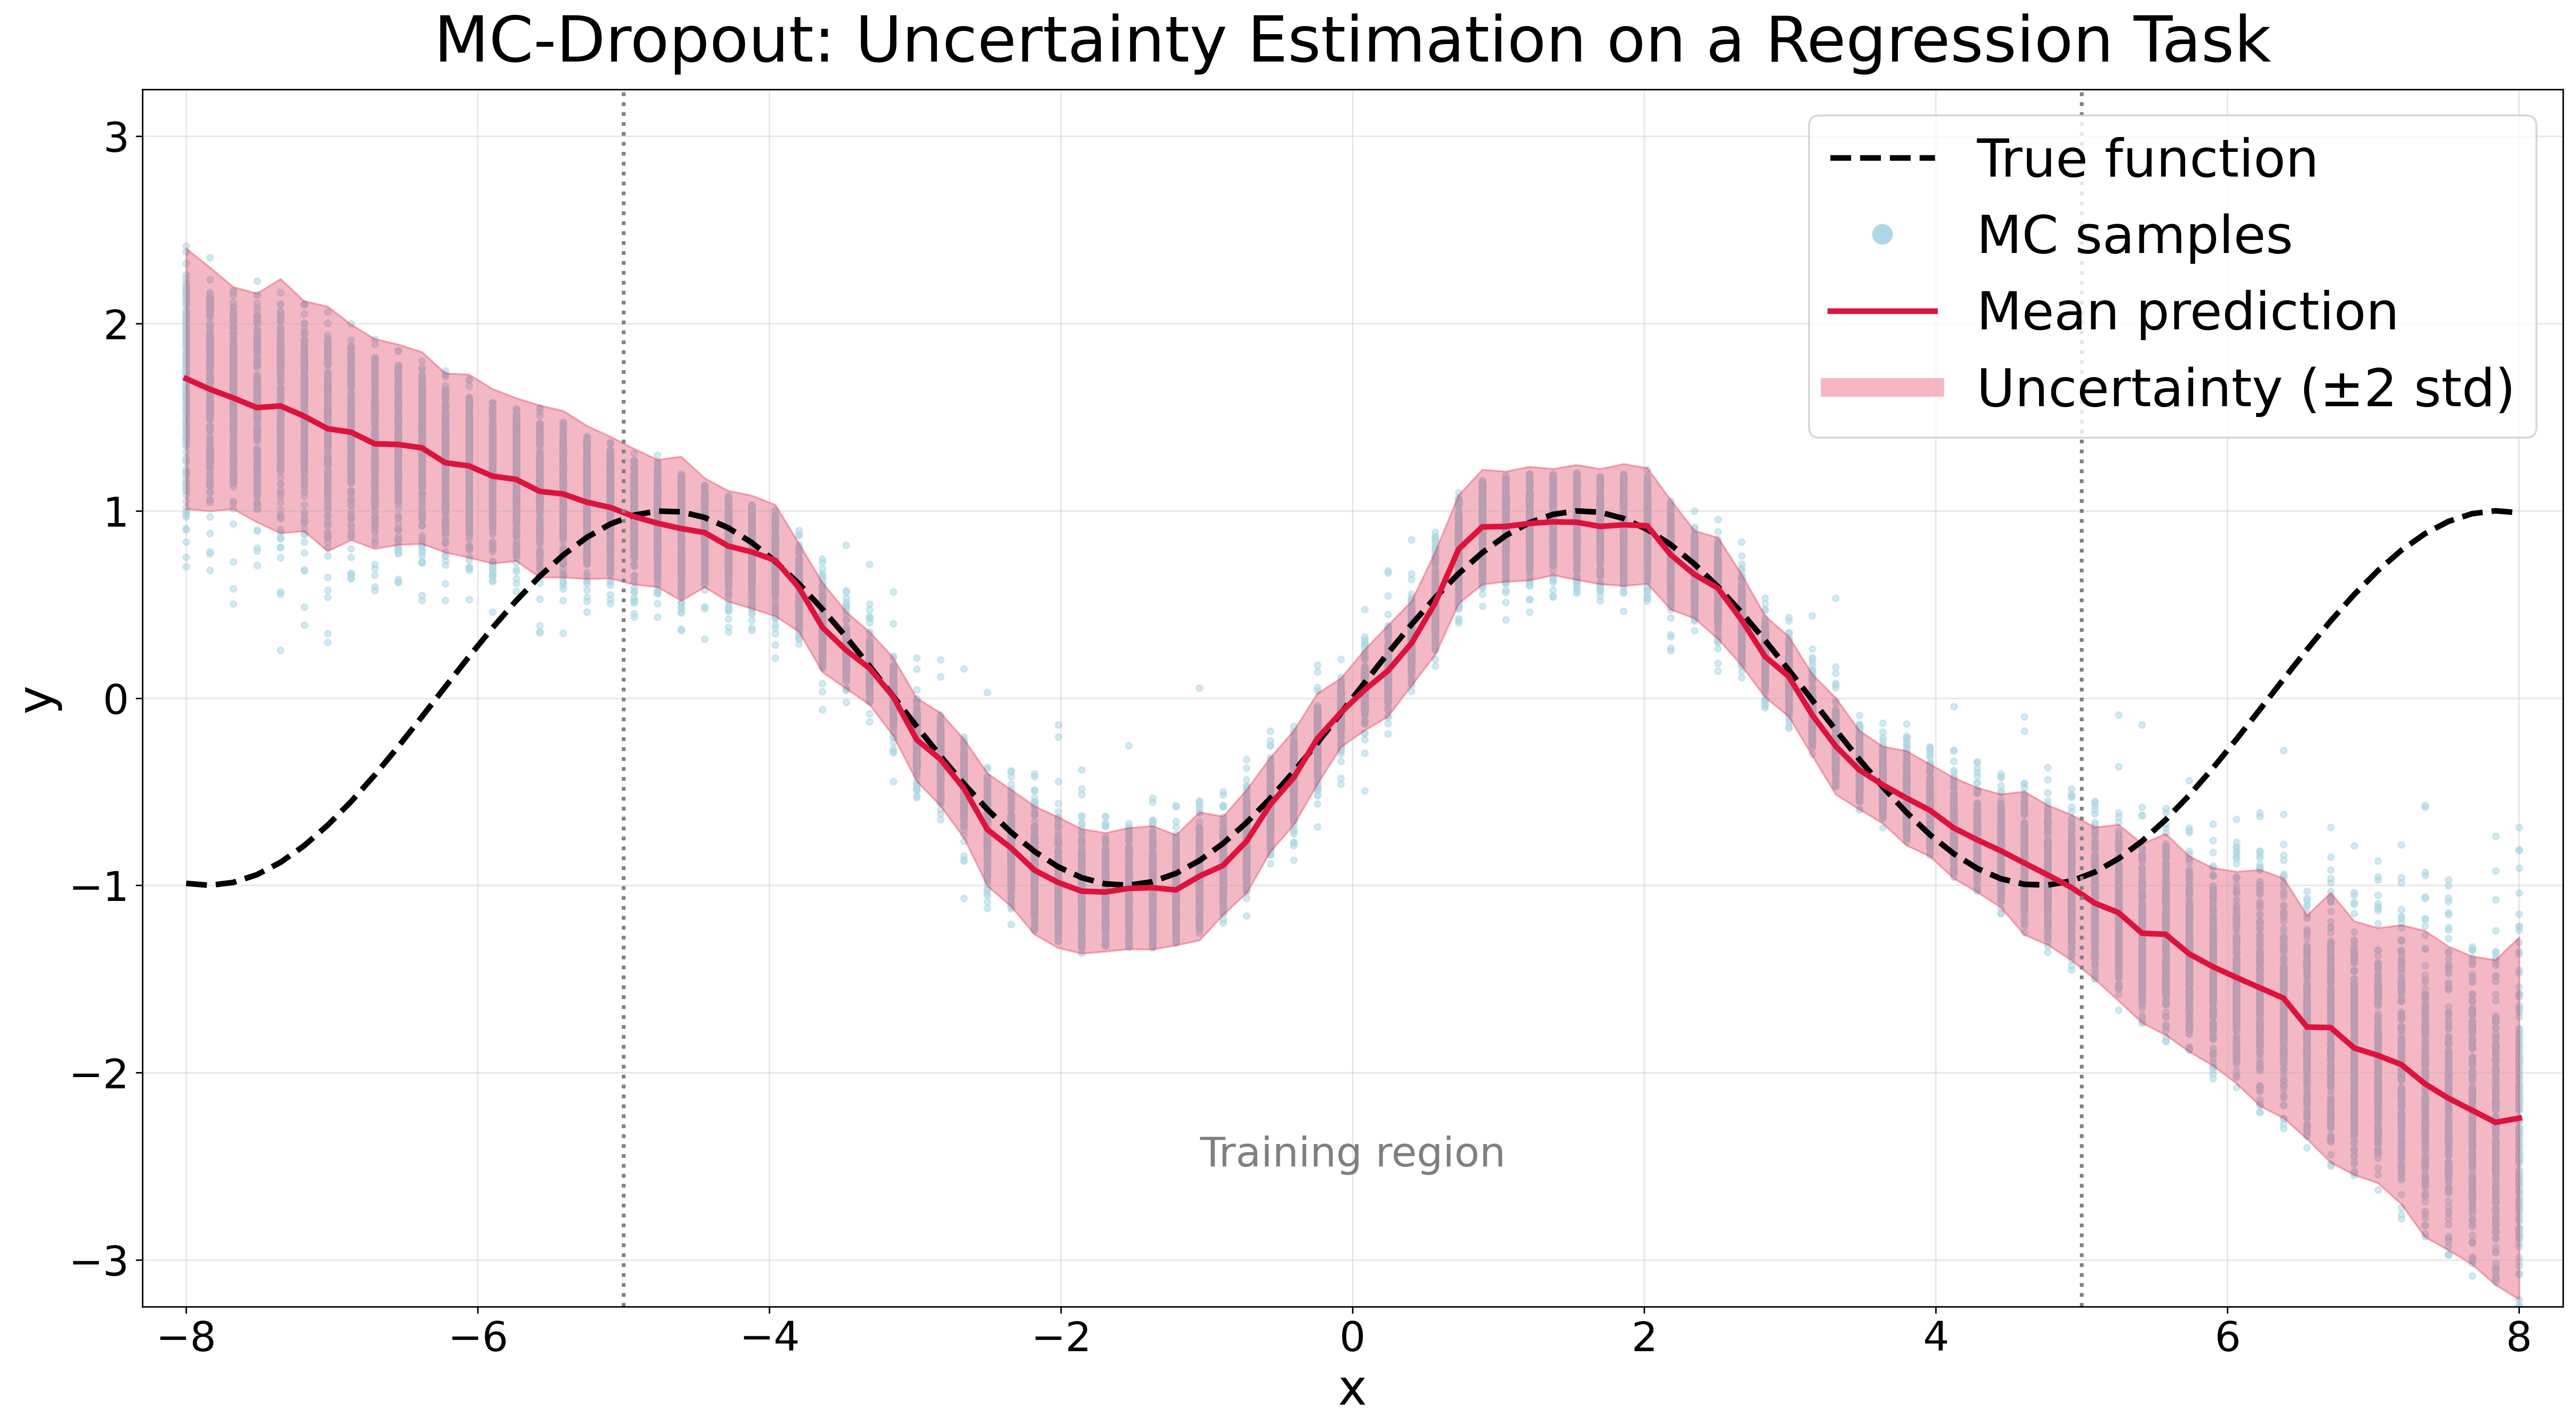
\includegraphics[width=\textwidth]{plots/mcd_regression.png}
  \end{subfigure}
  
  \vspace{0.3cm}
  \begin{subfigure}{0.8\textwidth}
    \centering
    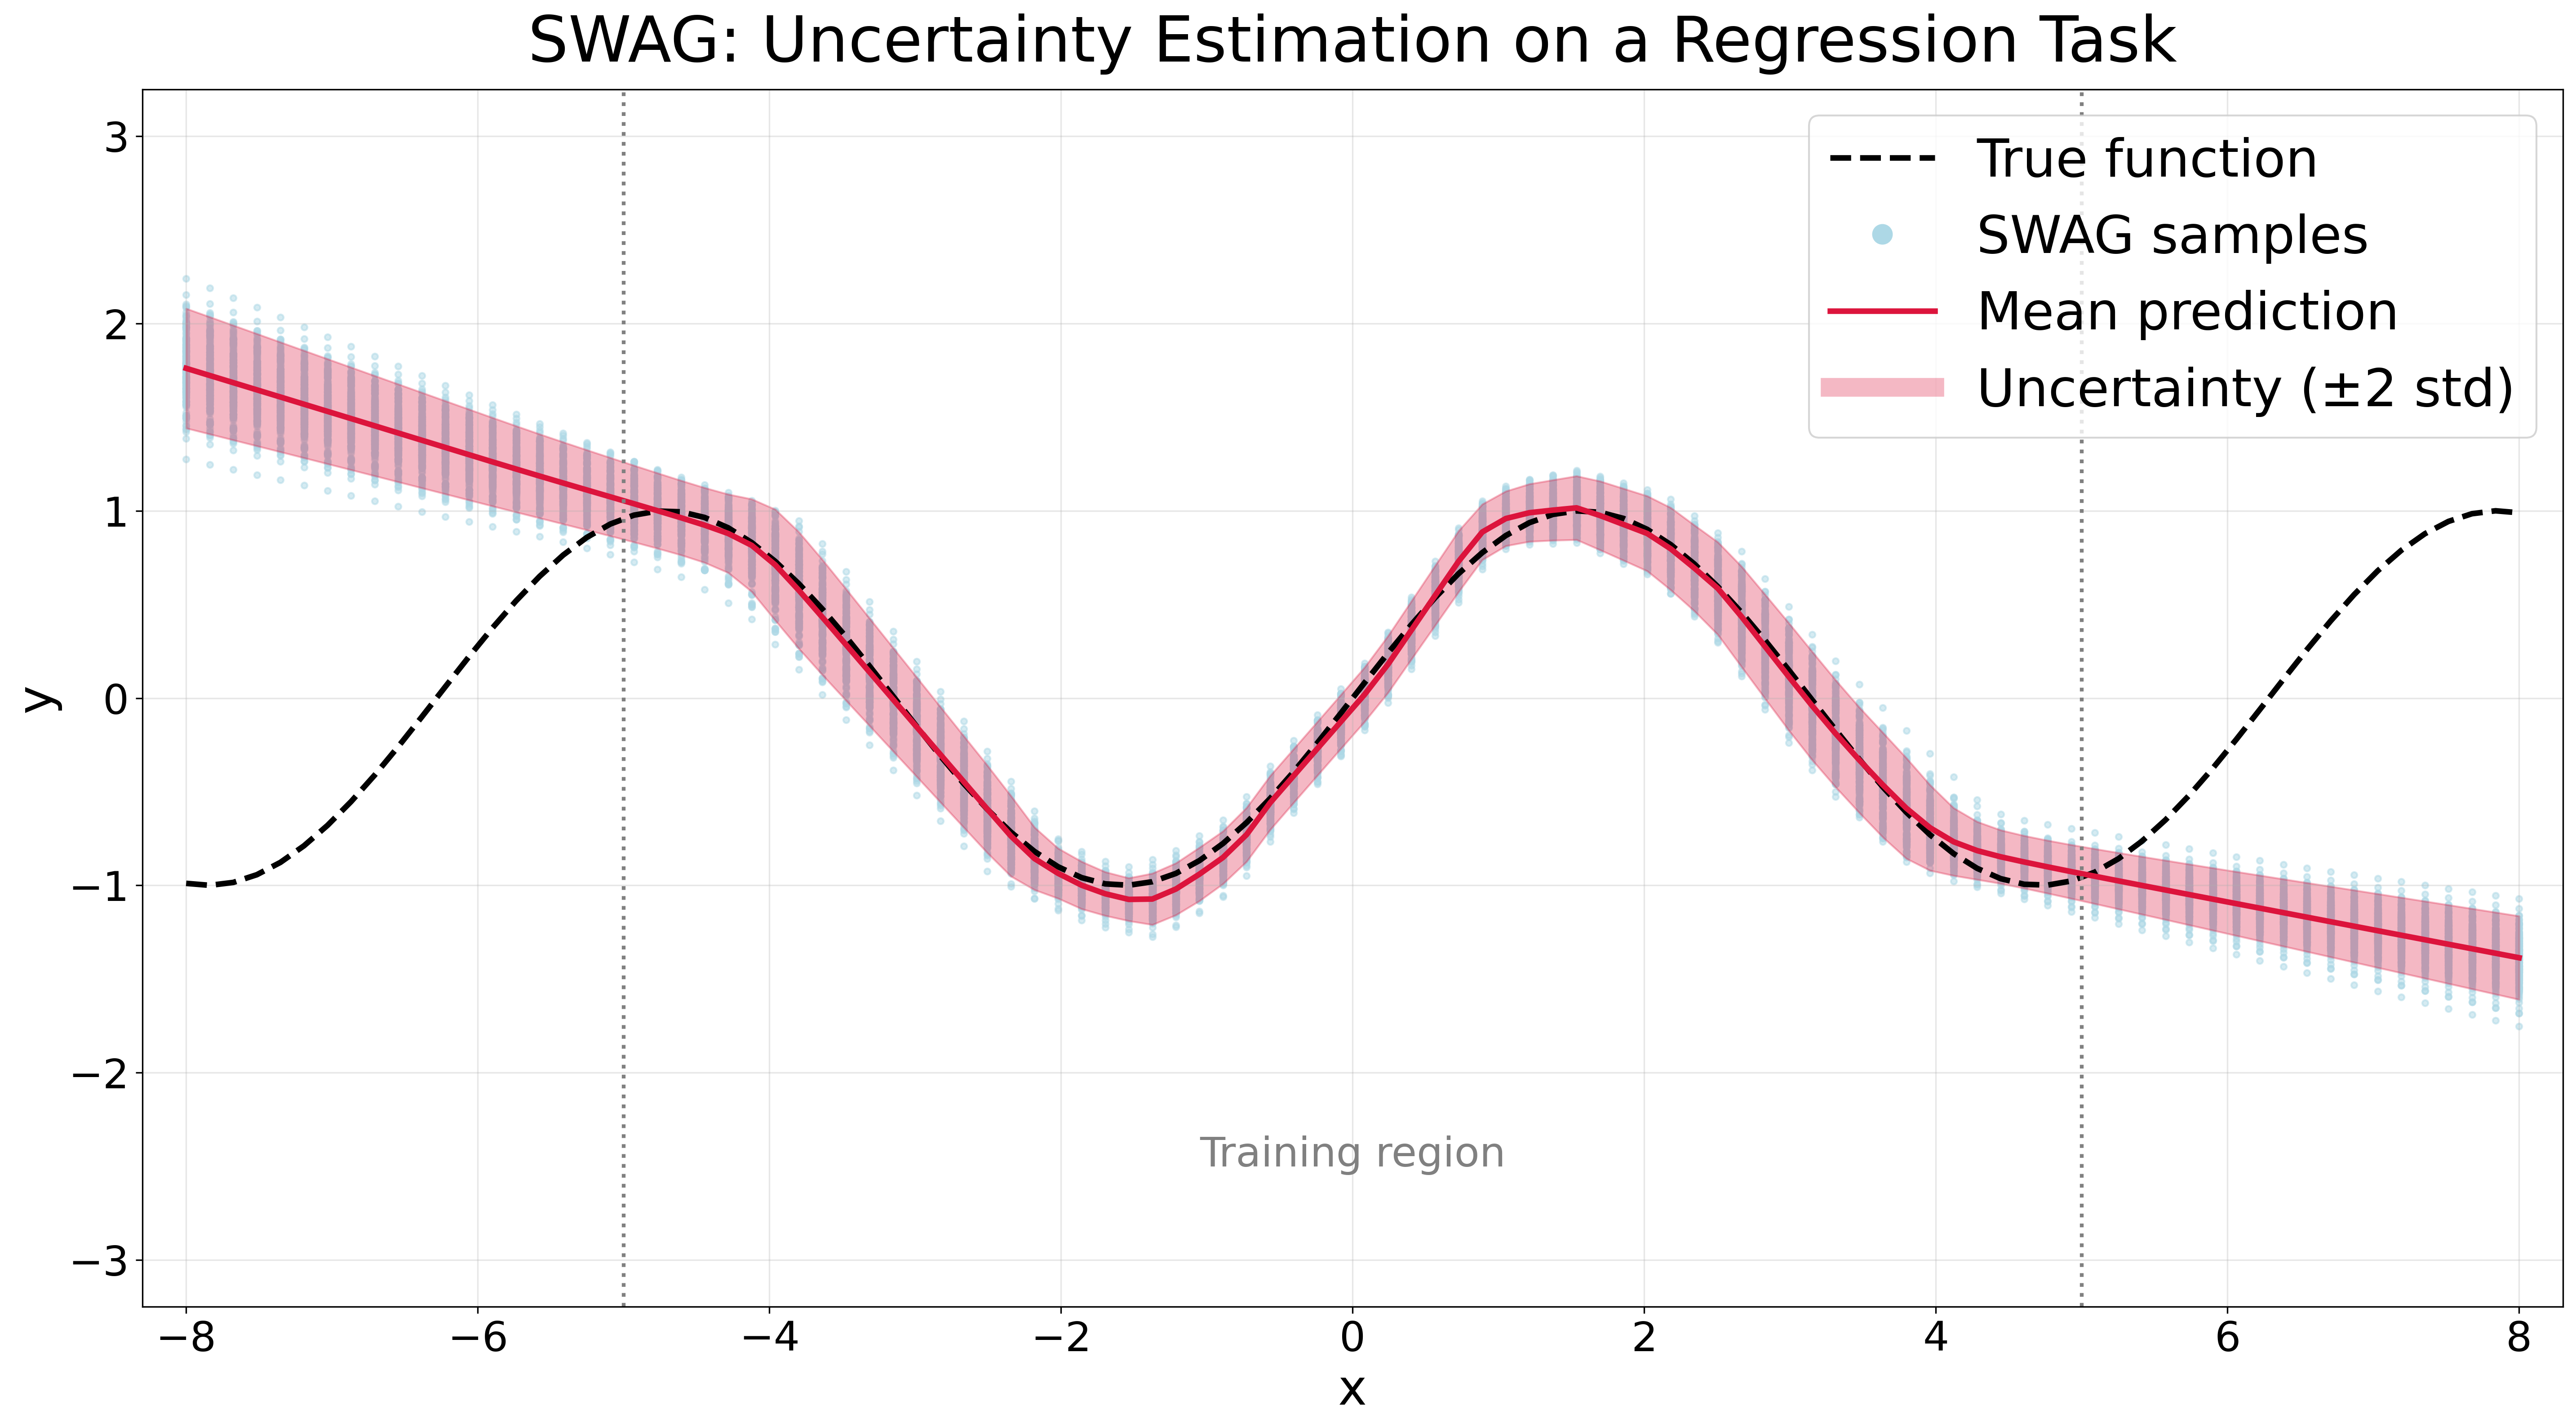
\includegraphics[width=\textwidth]{plots/swag_regression.png}
  \end{subfigure}
  \caption{Regression uncertainty estimation: MC-Dropout (top) and SWAG (bottom). Training domain ($|x| \leq 5$) marked by dashed lines.}
  \label{fig:regression}
\end{figure}

\FloatBarrier

\newpage
\paragraph{Classification Task}
The binary classification task uses a "two moons" dataset generated with scikit-learn \citep{scikit-learn}, it contains 500 training points with a nonlinear class boundary.

\vspace{0.15cm}
Figure \ref{fig:classification} shows both methods assign low uncertainty near training data, with sharp
decision boundaries (zone where the model transitions from predicting one class to the other). Both
increase predictive uncertainty in regions far from training data, successfully identifying OOD areas.
SWAG provides a smoother uncertainty estimation, while MC-Dropout produces a more scattered predictive
uncertainty, especially in the extrapolation region. 

Notably, some noisy points located in the wrong class' region (at approximately $(1.5, -0.5)$ and
$(0.5, 0.5)$) induce uncertainty spikes in SWAG but not MC-Dropout. This demonstrates SWAG's sensitivity
to weight-space perturbations \citep{izmailov2019swa}, as its covariance propagates uncertainty from
anomalies to neighboring regions. Near these noisy points, SWAG shows broader uncertainty intervals
while maintaining thinner boundaries elsewhere (e.g., near $(0,0)$).

\FloatBarrier

\begin{figure}[ht]
  \centering
  \begin{subfigure}{0.8\textwidth}
    \centering
    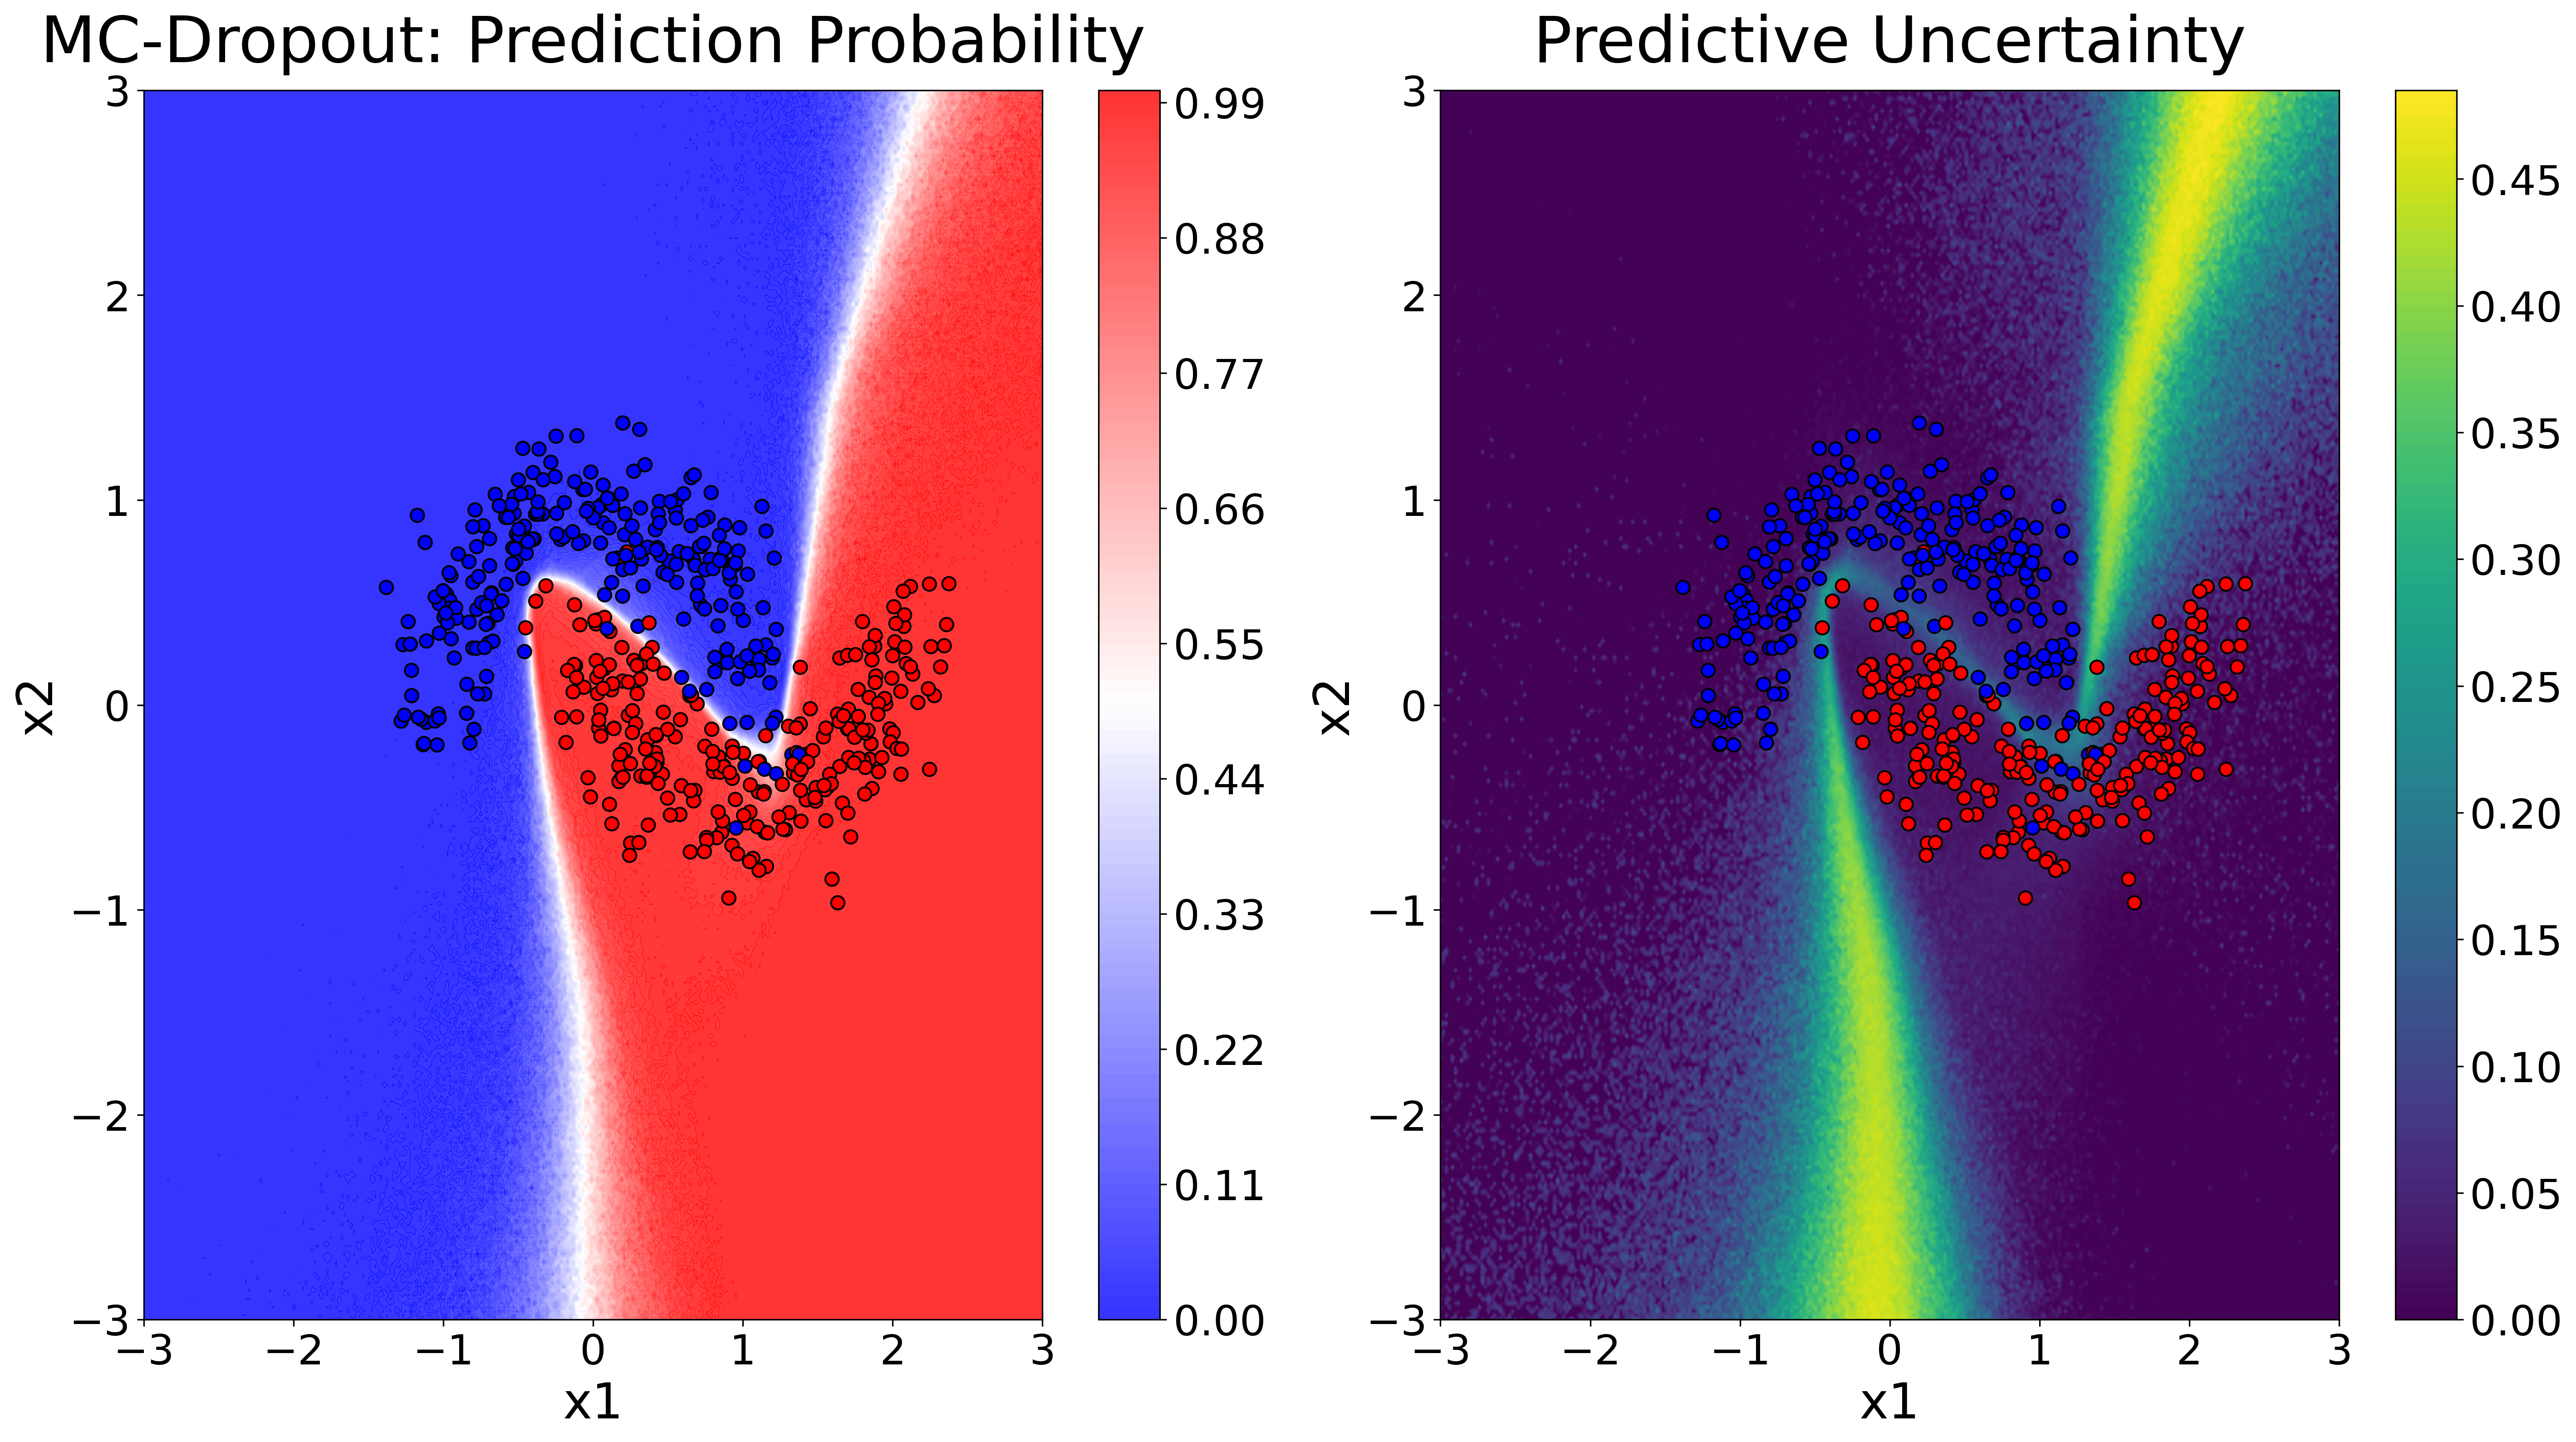
\includegraphics[width=\textwidth]{plots/mcd_classification.png}
  \end{subfigure}
  
  \vspace{0.3cm}
  \begin{subfigure}{0.8\textwidth}
    \centering
    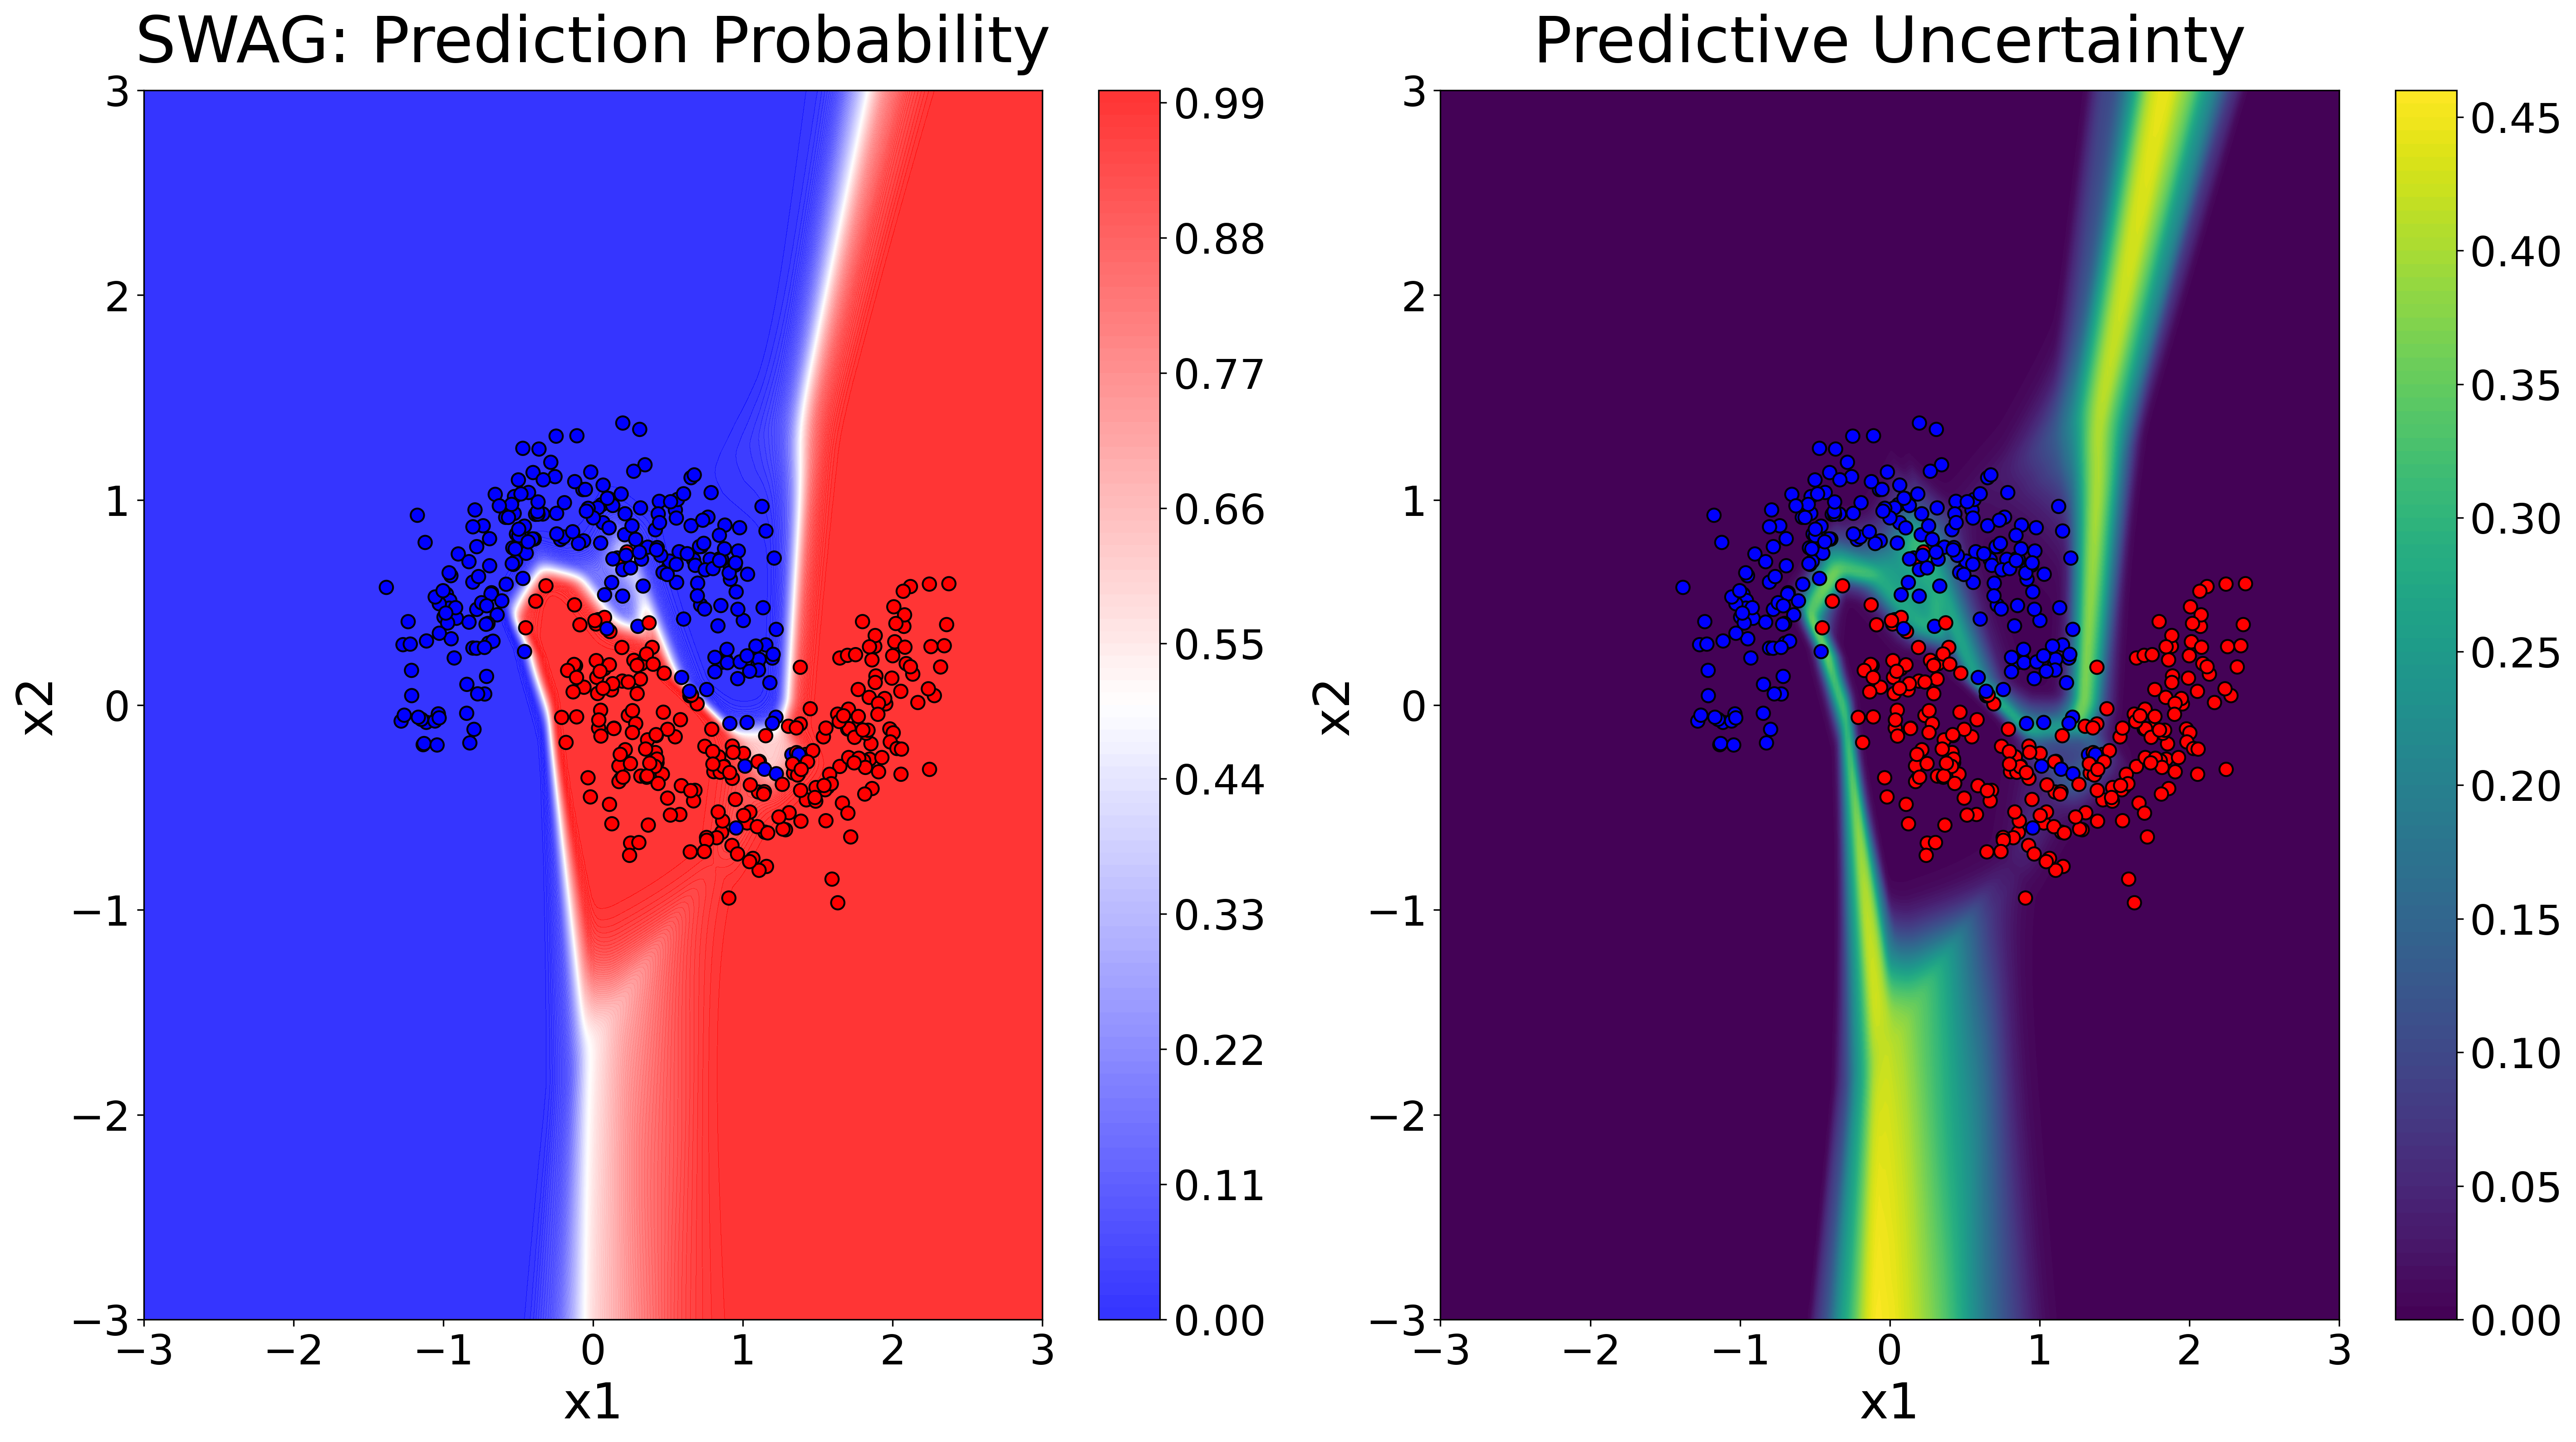
\includegraphics[width=\textwidth]{plots/swag_classification.png}
  \end{subfigure}
  \caption{Classification uncertainty: MC-Dropout (top) and SWAG (bottom). Color indicates true class (red/blue).}
  \label{fig:classification}
\end{figure}

\FloatBarrier



\newpage
\subsection{Evaluation on Real-world Data}
\label{exp:real-world_data}
To assess practical performance, the Boston Housing dataset is used \citep{harrison1978bh}.
It consists of 506 observations of housing prices in Boston suburbs. The response variable is the median
home value (in \$1000s), with features including crime rate, average rooms and highway accessibility.
Following ethical research standards, the racially problematic \texttt{B} variable is excluded.
It encoded the proportion of Black residents and reflected discriminatory assumptions in its original
formulation \citep[see, e.g.,][]{carlisle2020bh_ethicalIssue}.

\paragraph{Model Architecture and Training}
A neural network with four fully connected hidden layers is trained to predict standardized housing
prices. Hyperparameter tuning is conducted using a randomized grid search on a previously unseen
validation set. For MC-Dropout, dropout layers are once again added after each hidden layer.
Both models are trained using the Adam optimizer with a tuned learning rate and weight decay.

Table \ref{tab:bh_metrics} summarizes the evaluation results on the test set using three key metrics:
Root Mean Squared Error (RMSE) measures predictive accuracy (lower values preferred), Negative
Log-Likelihood (NLL) assesses uncertainty calibration (lower values indicate better calibration) and
Prediction Interval Coverage Probability (PICP) evaluates the reliability of 95\,\% uncertainty
intervals (values closer to 95\,\% reflect superior uncertainty estimation).

\begin{table}[h!]
\centering
\begin{tabular}{lccc}
\toprule
Method & RMSE & NLL & PICP (95\,\%) \\
\midrule
MC-Dropout & 0.4033 & 0.6814 & 0.7352 \\
SWAG       & 0.3947 & 0.2218 & 0.9314 \\
\bottomrule
\end{tabular}
\caption{Test performance on the Boston Housing dataset.}
\label{tab:bh_metrics}
\end{table}

Both methods achieve comparable point-prediction accuracy, as evidenced by their similar RMSE values.
However, SWAG demonstrates significantly better uncertainty calibration, with a much lower NLL and a
near-ideal PICP of 93.14\,\%. MC-Dropout's PICP of 73.52\,\% indicates systematic undercoverage.
The notable discrepancy in NLL values further reveals MC-Dropout's tendency toward overconfidence,
as it frequently assigns high certainty to incorrect predictions.


\paragraph{Uncertainty Behavior Analysis}
Figure \ref{fig:bh_uncertainty_comp2x2} provides a comparative analysis of uncertainty characteristics between MC-Dropout and SWAG.

The top-left subplot displays histograms of predictive standard deviations, revealing distinct
distributional profiles. MC-Dropout exhibits a sharp peak near 0.16, indicating overconfident estimates
with limited variability, whereas SWAG generates a broader distribution centered near 0.2 with an
extended right tail, reflecting more moderate and diverse uncertainty quantification.

In the top-right scatter plot of absolute residuals versus predictive standard deviations, SWAG displays a
wider vertical spread of points, suggesting that it assigns greater uncertainty to predictions with larger
errors. On the other hand, MC-Dropout's points are more tightly clustered near the origin, indicating
uniformly low uncertainty estimates even when residuals are non-negligible. This pattern reinforces the
impression of overconfidence in MC-Dropout's uncertainty outputs.

The bottom row consists of two calibration plots, where predicted means are plotted against true target
values and shaded confidence bands represent 95\,\% predictive intervals. While both models align well
along the identity line in high-density regions, SWAG produces slightly wider confidence bands. This
demonstrates more conservative and better-calibrated uncertainty estimates.

\FloatBarrier

\begin{figure}[ht]
    \centering
    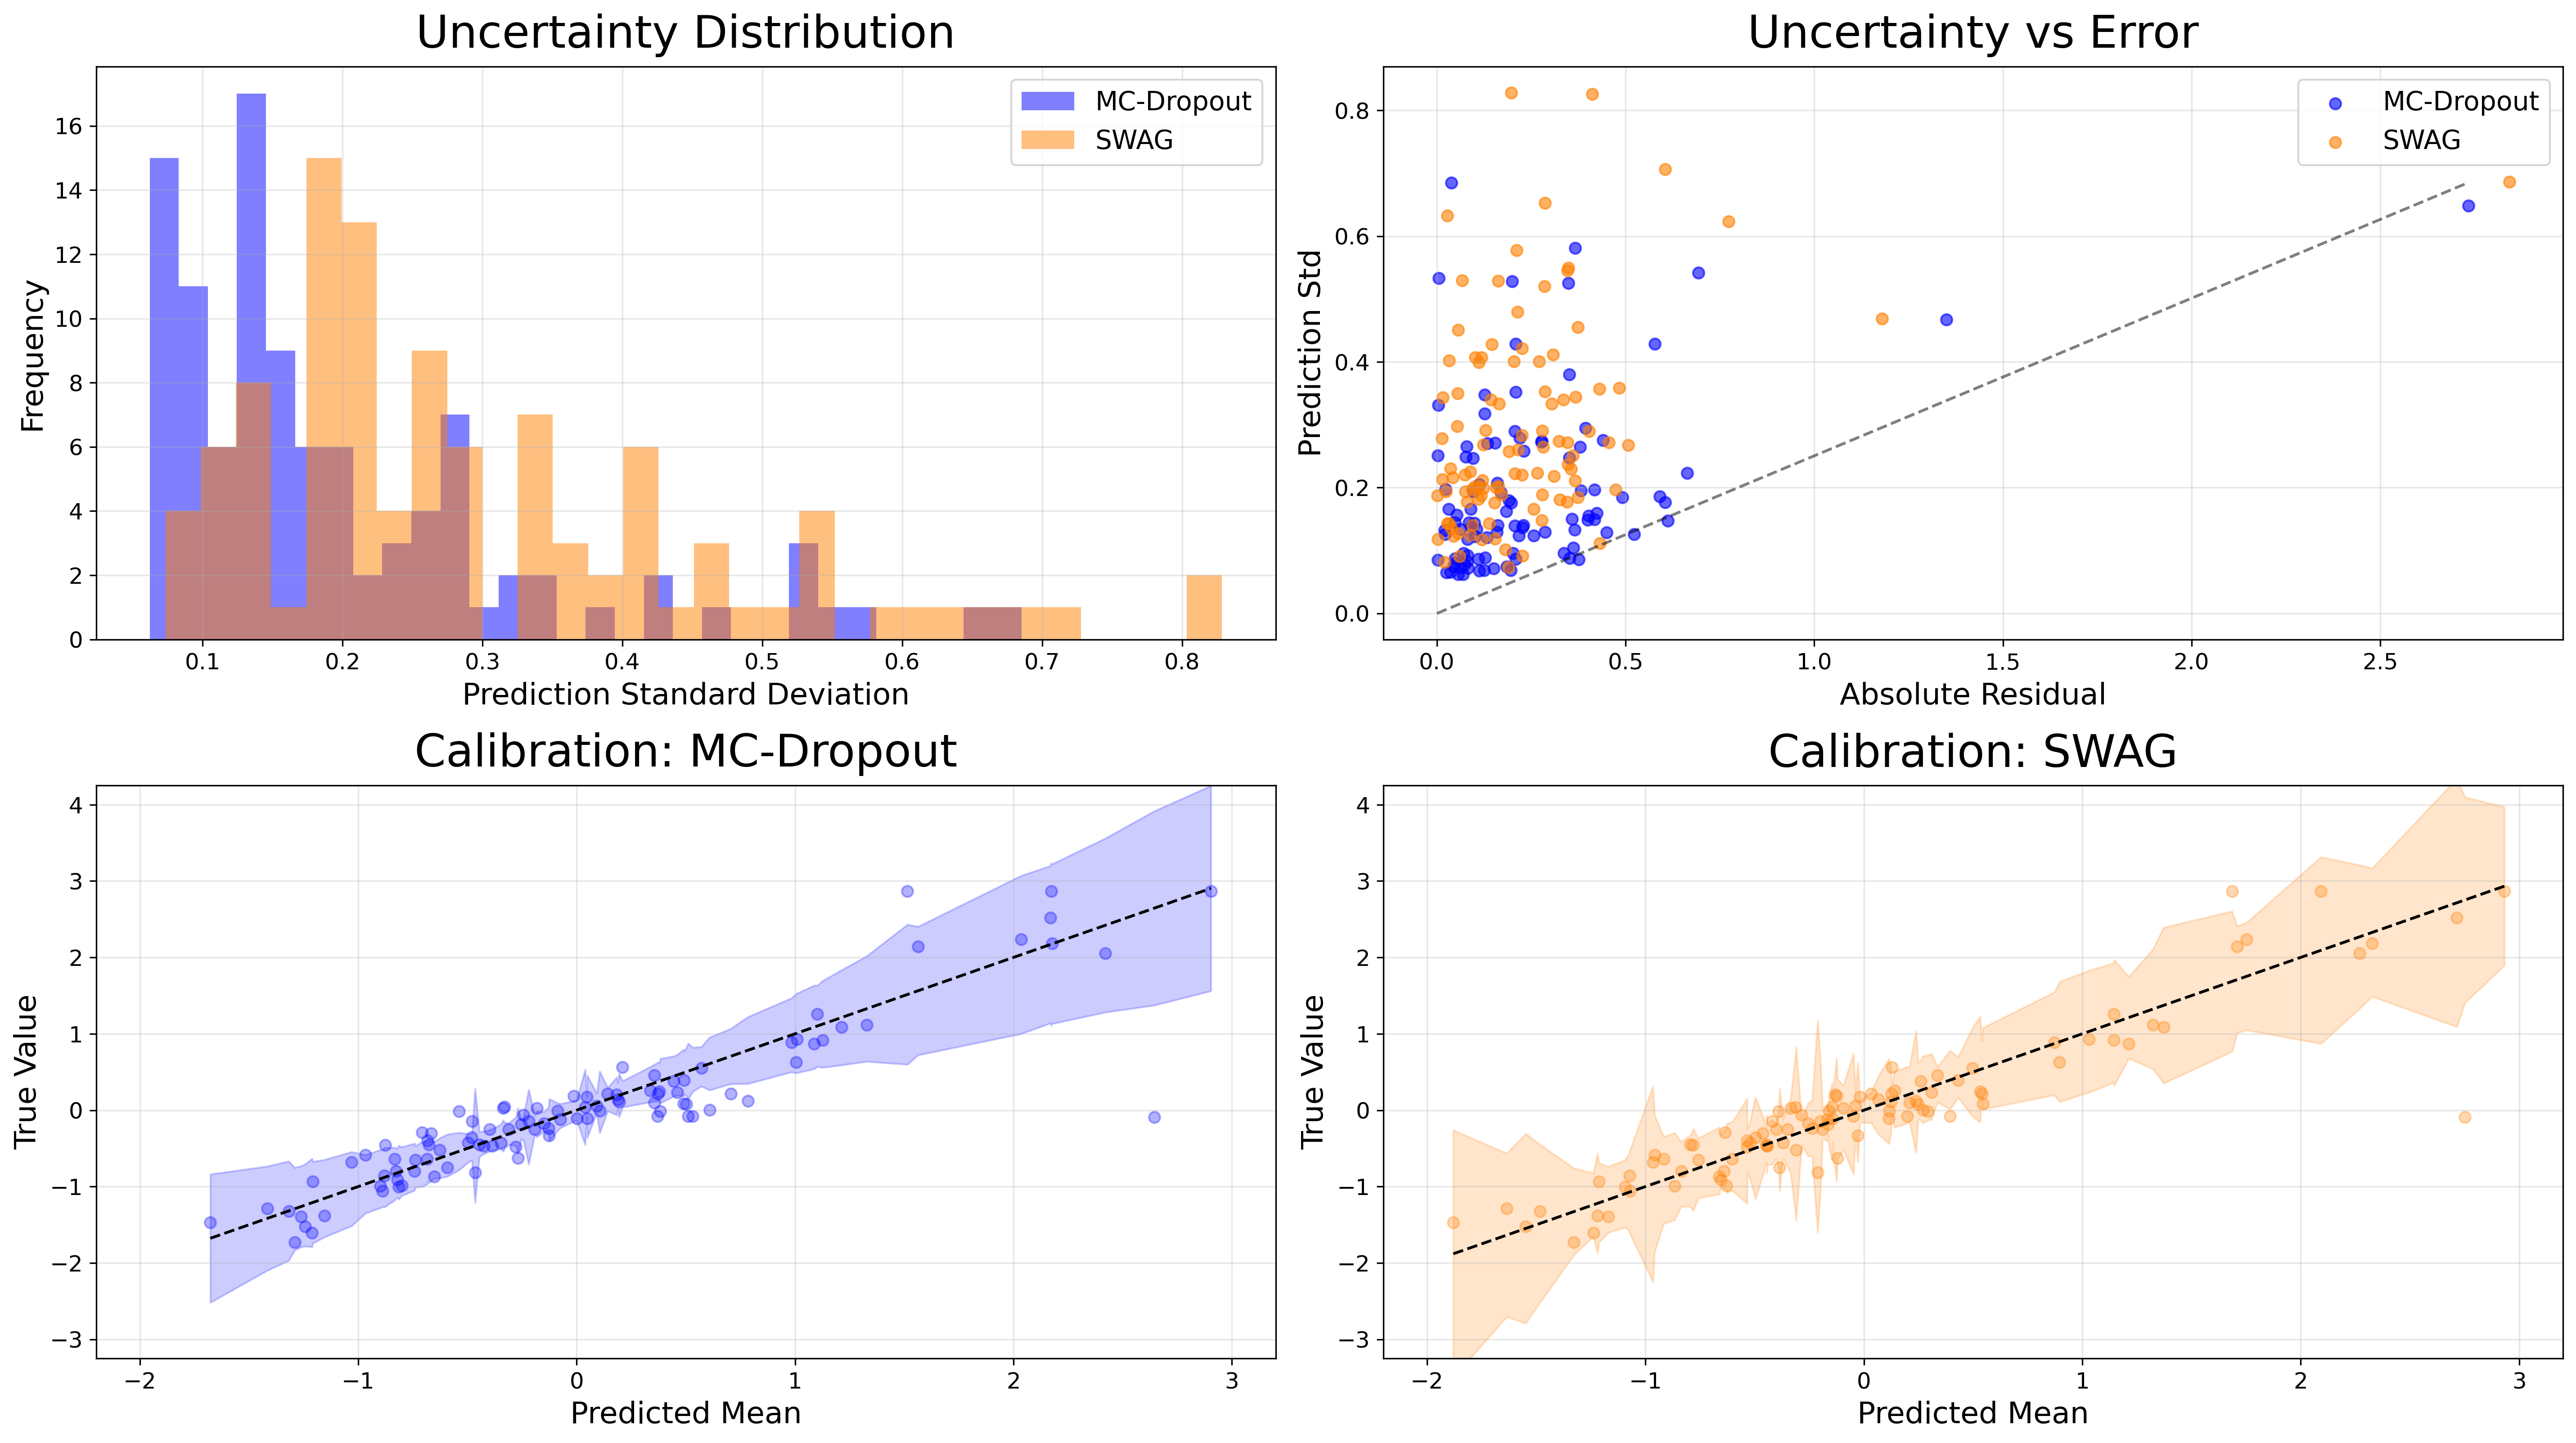
\includegraphics[width=0.9\linewidth]{plots/bh_uncertainty_comp2x2.png}
    \caption{Comparison of uncertainty behaviors for MC-Dropout and SWAG on the Boston Housing dataset.}
    \label{fig:bh_uncertainty_comp2x2}
\end{figure}

\FloatBarrier


\paragraph{Out-of-Distribution Analysis}
To evaluate the robustness of uncertainty estimation under distribution shift, two types of
out-of-distribution (OOD) scenarios are examined. Natural OOD samples with exceptionally high median
income (\texttt{MedInc}) and artificially perturbed samples with amplified income and reduced occupancy.
Table~\ref{tab:ood_results} displays predictive accuracy (RMSE) and uncertainty calibration (NLL) across
in-domain and OOD conditions.

\begin{table}[h!]
\centering
\begin{tabular}{lccccc}
\toprule
 & \multicolumn{2}{c}{MC-Dropout} & \multicolumn{2}{c}{SWAG} \\
Scenario & RMSE & NLL & RMSE & NLL \\
\midrule
In-domain & 0.4033 & 0.6814 & 0.3947 & 0.2218 \\
Natural OOD & 0.2768 & 0.2331 & 0.3838 & 0.6708 \\
Artificial OOD & 0.4283 & 0.7249 & 0.4094 & 0.3006 \\
\bottomrule
\end{tabular}
\caption{OOD performance comparison.}
\label{tab:ood_results}
\end{table}

For natural OOD samples, MC-Dropout shows point-prediction accuracy with the RMSE decreasing from 0.4033 to
0.2768, but exhibits a substantial NLL reduction (0.6814 to 0.2331). This divergence suggests potentially
overconfident uncertainty estimates that fail to properly reflect distribution shift. In contrast, SWAG
maintains stable predictive accuracy (RMSE: 0.3947 to 0.3838) while appropriately increasing NLL (0.2218
to 0.6708), indicating more cautious uncertainty estimation under distribution shift.

In the artificial OOD scenario, both methods show degraded performance. MC-Dropout's RMSE increases to
0.4283 and NLL to 0.7249, while SWAG's RMSE increases to 0.4094 and NLL to 0.3006. The increased NLL
indicates worse uncertainty calibration compared to in-domain samples and SWAG maintains its superior
calibration. Both methods show a very similar relative response under artificial perturbations.

Figure \ref{fig:bh_ood_comp} complements the tabular metrics by visualizing the distribution of predictive
standard deviations (i.e., uncertainty) shifts between in-domain and artificial OOD conditions. For MC-Dropout (left panel), the histogram shows negligible distributional change with marginally
increased maximum uncertainty, indicating limited responsiveness to distribution shift. SWAG (right panel)
displays a substantial increase in maximum uncertainty (33\,\%), this demonstrates that SWAG has the
capacity to effectively register distributional changes and inflate uncertainty accordingly
\citep{maddox2019swag}.

\FloatBarrier

\begin{figure}[ht]
    \centering
    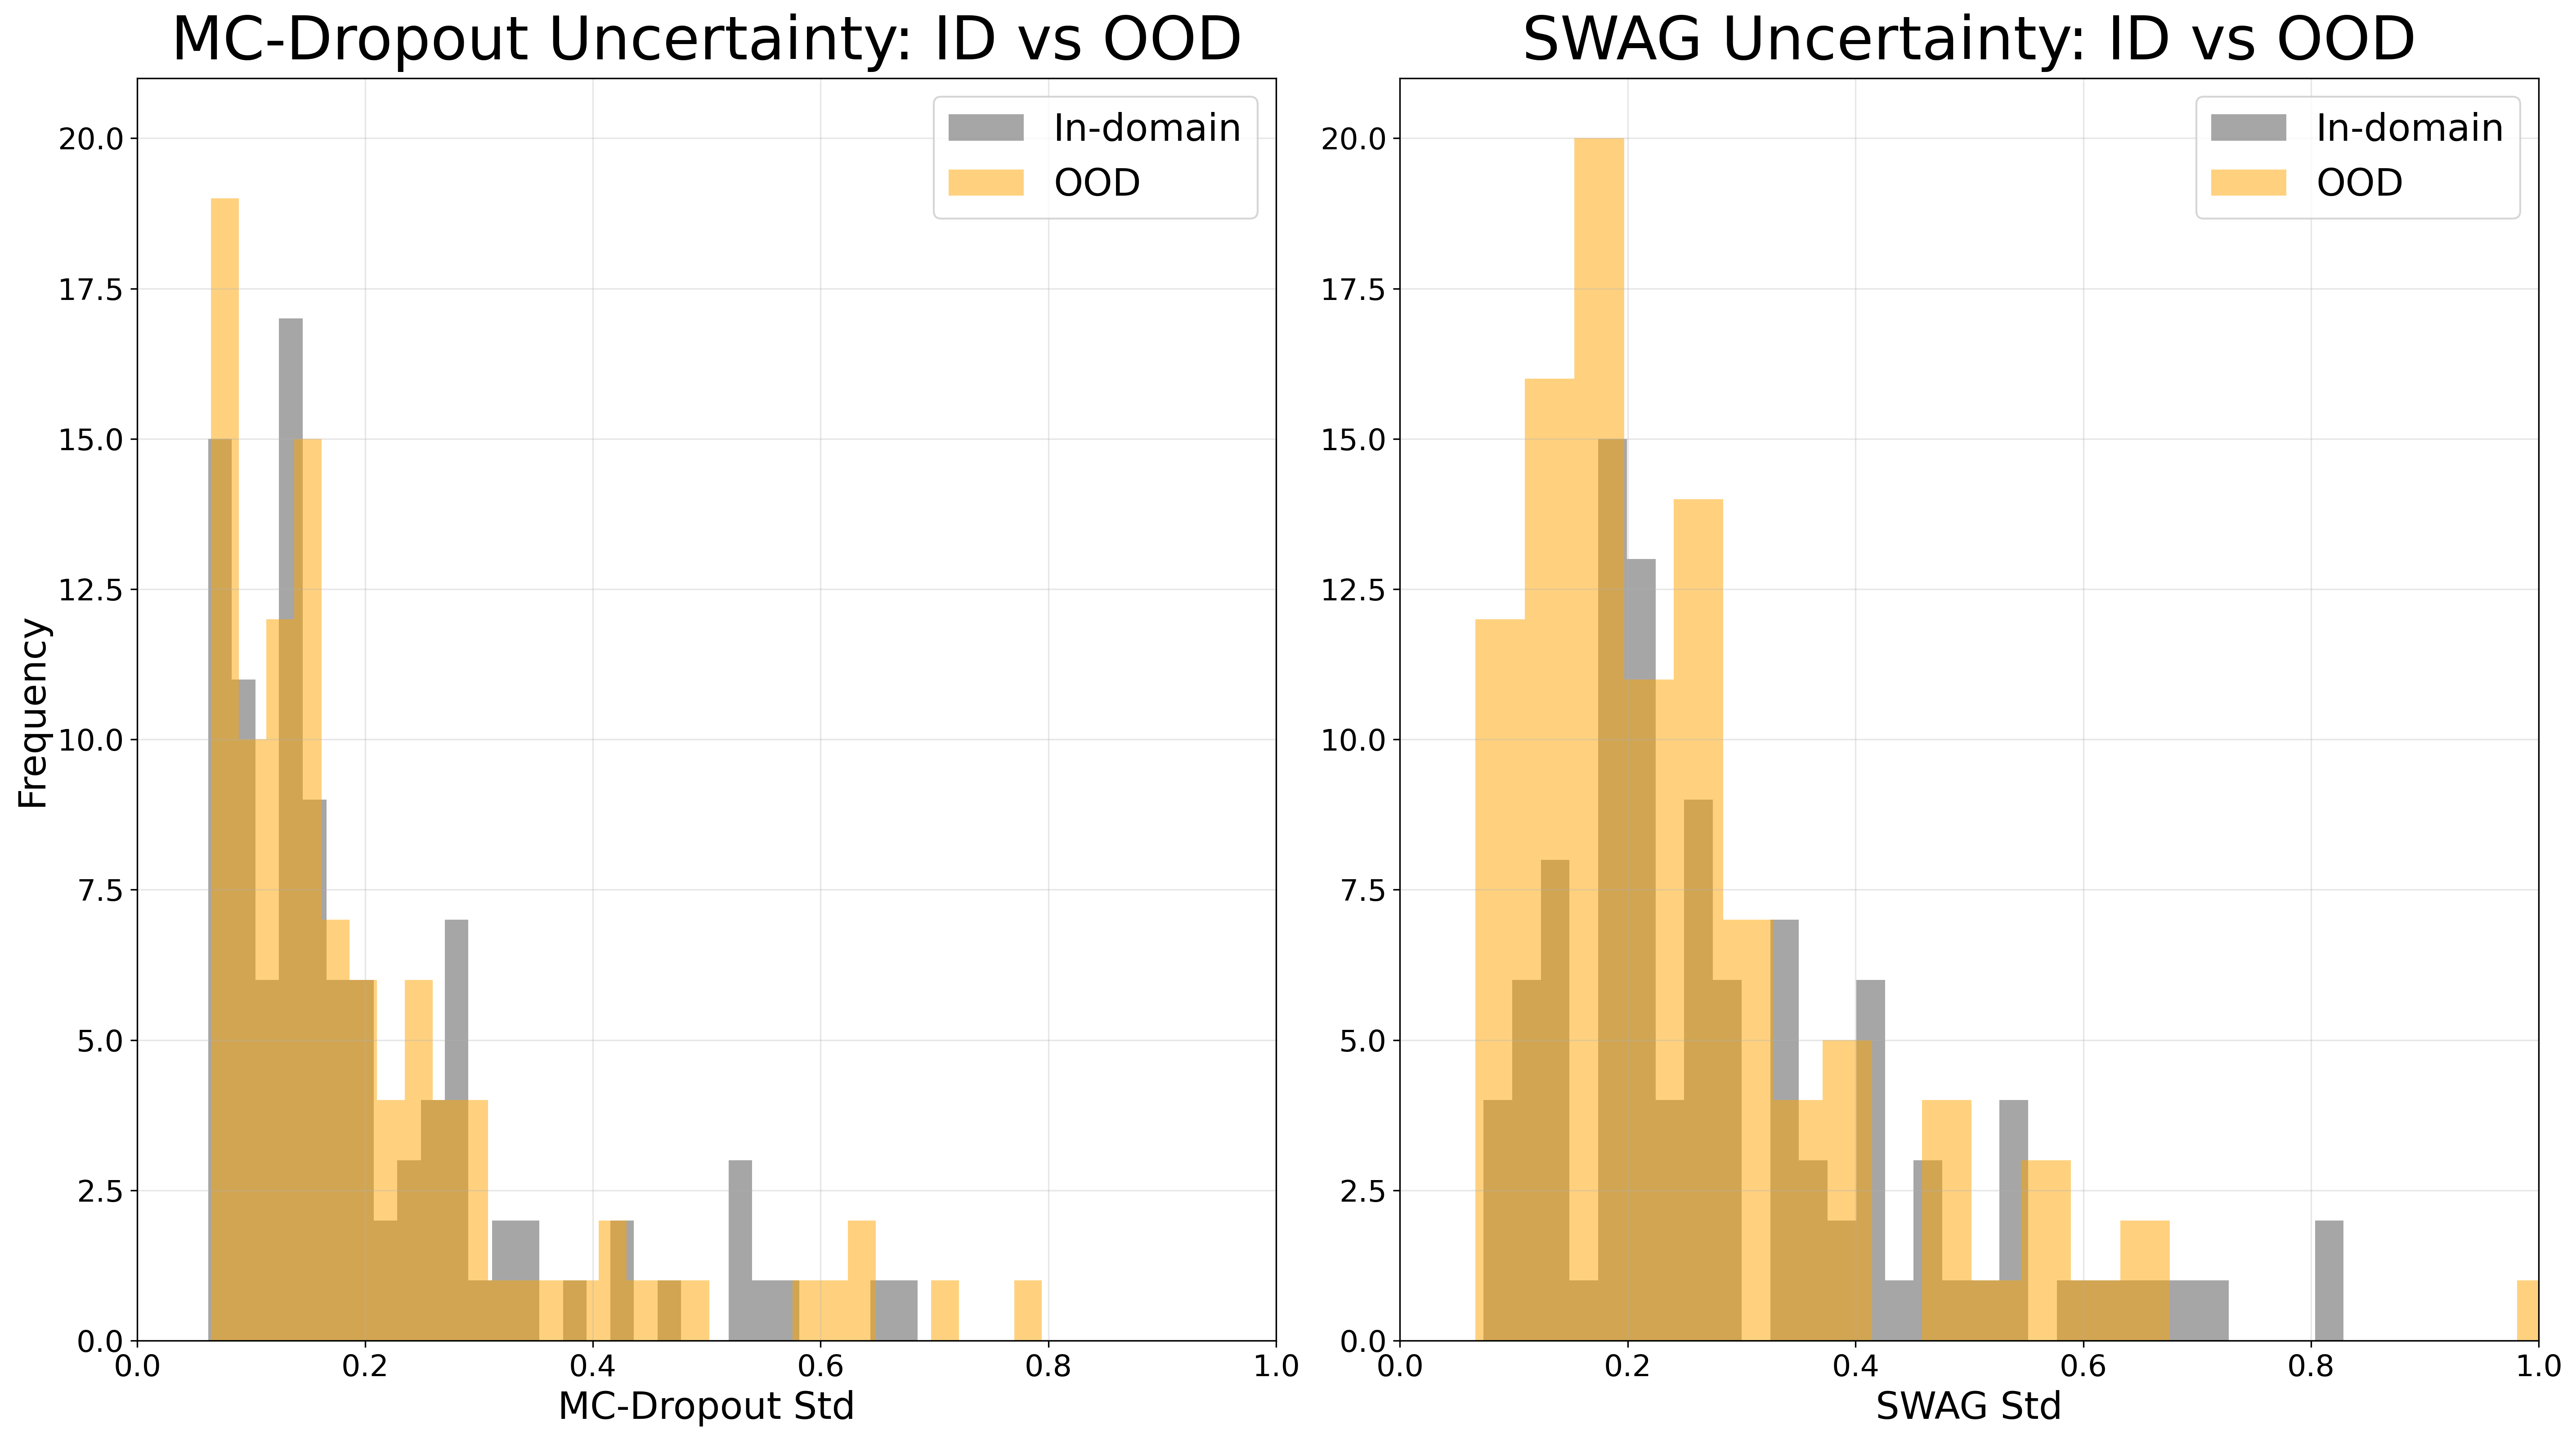
\includegraphics[width=0.9\linewidth]{plots/bh_ood_comp.png}
    \caption{Uncertainty comparison between in-domain and out-of-distribution (OOD) samples for MC-Dropout (left) and SWAG (right).}
    \label{fig:bh_ood_comp}
\end{figure}

\FloatBarrier

The Boston Housing evaluation demonstrates distinct characteristics between SWAG and MC-Dropout.
Both methods achieve comparable point-prediction accuracy, but SWAG exhibits superior uncertainty
calibration as evidenced by lower NLL and near-ideal PICP. Uncertainty visualization reveals SWAG's more
diverse uncertainty distribution and stronger error-uncertainty correlation. Under distribution shift,
SWAG maintains stable accuracy while appropriately inflating uncertainty, whereas MC-Dropout shows
concerning overconfidence.

\newpage

\section{Discussion}
\label{discussion}

This work systematically compares MC-Dropout and SWAG for uncertainty quantification, revealing a
fundamental trade-off between computational efficiency and and the quality of uncertainty estimates.
MC-Dropout's advantages lie in computational efficiency, generating uncertainty estimates through simple
stochastic forward passes. It however shows limitations including undercoverage and overconfidence under
distribution shift. SWAG addresses these issues through SGD-based weight-space exploration, yielding
better-calibrated uncertainties with improved responsiveness to distributional changes, but requiring
extended training and increased memory overhead.

\vspace{0.15cm}
Given these differences, our findings suggest practical recommendations for choosing between MC-Dropout and
SWAG. MC-Dropout suits applications prioritizing speed and simplicity where uncertainties play a secondary
role, particularly in stable environments. Its deficient OOD performance (Table \ref{tab:ood_results})
makes it unsuitable for safety-critical systems. SWAG proves preferable when the reliability of uncertainty
is central to decision making, especially where training budget permits extended exploration and deployment
contexts involve potential distribution shifts.

\vspace{0.15cm}
Looking ahead, both methods present opportunities for improvement. Extensions of MC-Dropout could reduce
its overconfidence through techniques such as Concrete Dropout \citep{gal2017concretedropout}, which learns
layer-specific retention probabilities to better calibrate uncertainty. SWAG can be further improved in
terms of expressiveness and efficiency. MultiSWAG \citep{onal2024multiswag}, for instance, ensemble the
several independently trained SWAG models to approximate multimodal posteriors, while SWALP
\citep{yang2019swalp} enables low-precision inference, reducing computational cost without degrading
performance. For applications where multimodality capture is essential, Deep Ensembles
\citep{lakshminarayanan2017preduncw/deepensembles} remain superior despite high computational costs,
with MultiSWAG offering a promising balance between efficiency and robustness.

\vspace{0.15cm}
The selection of an uncertainty quantification method should ultimately be guided by the specific
requirements of the target application. MC-Dropout is well suited for lightweight and scalable solutions,
SWAG for reliable calibration, and ensemble variants where resources permit robust uncertainty modeling.

\newpage

\section{Conclusion}
\label{conclusion}

Through rigorous evaluation across synthetic and real-world datasets, this work has illustrated a
fundamental trade-off in uncertainty estimation quality between MC-Dropout and SWAG. The systematic
comparison reveals distinct characteristics that guide practical method selection.

\vspace{0.15cm}
Our experiments demonstrate that both methods effectively capture predictive uncertainty within their
training distribution. In synthetic tasks (Figures \ref{fig:regression}, \ref{fig:classification}),
they successfully identify out-of-distribution regions while maintaining accurate in-domain predictions.
SWAG produced smoother uncertainty estimates in both regression and classification tasks, while MC-Dropout
yielded noisier predictions. In the regression task specifically, MC-Dropout generated more conservative
uncertainty intervals.

When applied to the Boston Housing dataset (Section \ref{exp:real-world_data}), critical differences
emerged. SWAG produced better-calibrated uncertainty estimates, achieving near-ideal prediction interval
coverage (Table \ref{tab:bh_metrics}) and appropriately increasing uncertainty under distributional changes
(Table \ref{tab:ood_results}). MC-Dropout showed undercoverage and concerning overconfidence in OOD
scenarios. SWAG's uncertainty distributions showed greater diversity and stronger error correlation
(Figure \ref{fig:bh_uncertainty_comp2x2}), while providing more reliable confidence intervals.

\vspace{0.15cm}
Ultimately, this work demonstrates that Bayesian approximations don't need to sacrifice practical utility,
as both methods provide valuable uncertainty estimates, with SWAG offering superior calibration at
moderately higher computational overhead. As neural networks increasingly support critical decision-making,
selecting appropriate uncertainty quantification methods becomes essential for developing trustworthy AI
systems.


\newpage


% ------------------------------------------------------------------------------
% APPENDIX ---------------------------------------------------------------------
% ------------------------------------------------------------------------------
    
\pagenumbering{Roman}

\setcounter{page}{16} % CHANGE

\appendix

\section{Appendix}
\label{app}

\subsection{Usage of AI}

OpenAI’s free LLM, ChatGPT-4o, was used to improve the grammar and wording in this work and to document the code. It also assisted in understanding the implementation of SWAG as described by \citet{maddox2019swag} (\url{https://github.com/wjmaddox/swa_gaussian/}). The tool was used to aid editorial refinements and technical understanding, not to generate original research content.


\subsection{Additional plots}

\paragraph{Tuned NN on synthetic regression and classification}
This appendix presents uncertainty estimates from the same model architectures used in Section
\ref{exp:synthetic}, now with optimized hyperparameters. Figures \ref{fig:regression_tuned} and
\ref{fig:classification_tuned} show uncertainty visualizations comparable to their non-tuned counterparts
in Figures \ref{fig:regression} and \ref{fig:classification}.

In the regression task (Figure \ref{fig:regression_tuned}), both methods exhibit visibly reduced
uncertainty compared to non-tuned results, evidenced by tighter confidence intervals throughout the domain.
For classification (Figure \ref{fig:classification_tuned}), SWAG shows substantially thinner uncertainty
estimates across the input space. MC-Dropout, however, maintains nearly identical uncertainty patterns to
its non-tuned version, with only subtle adjustments to the decision boundary attributable to improved model
performance rather than changes in uncertainty quantification behavior.

\FloatBarrier

\begin{figure}[ht]
  \centering
  \begin{subfigure}{0.8\textwidth}
    \centering
    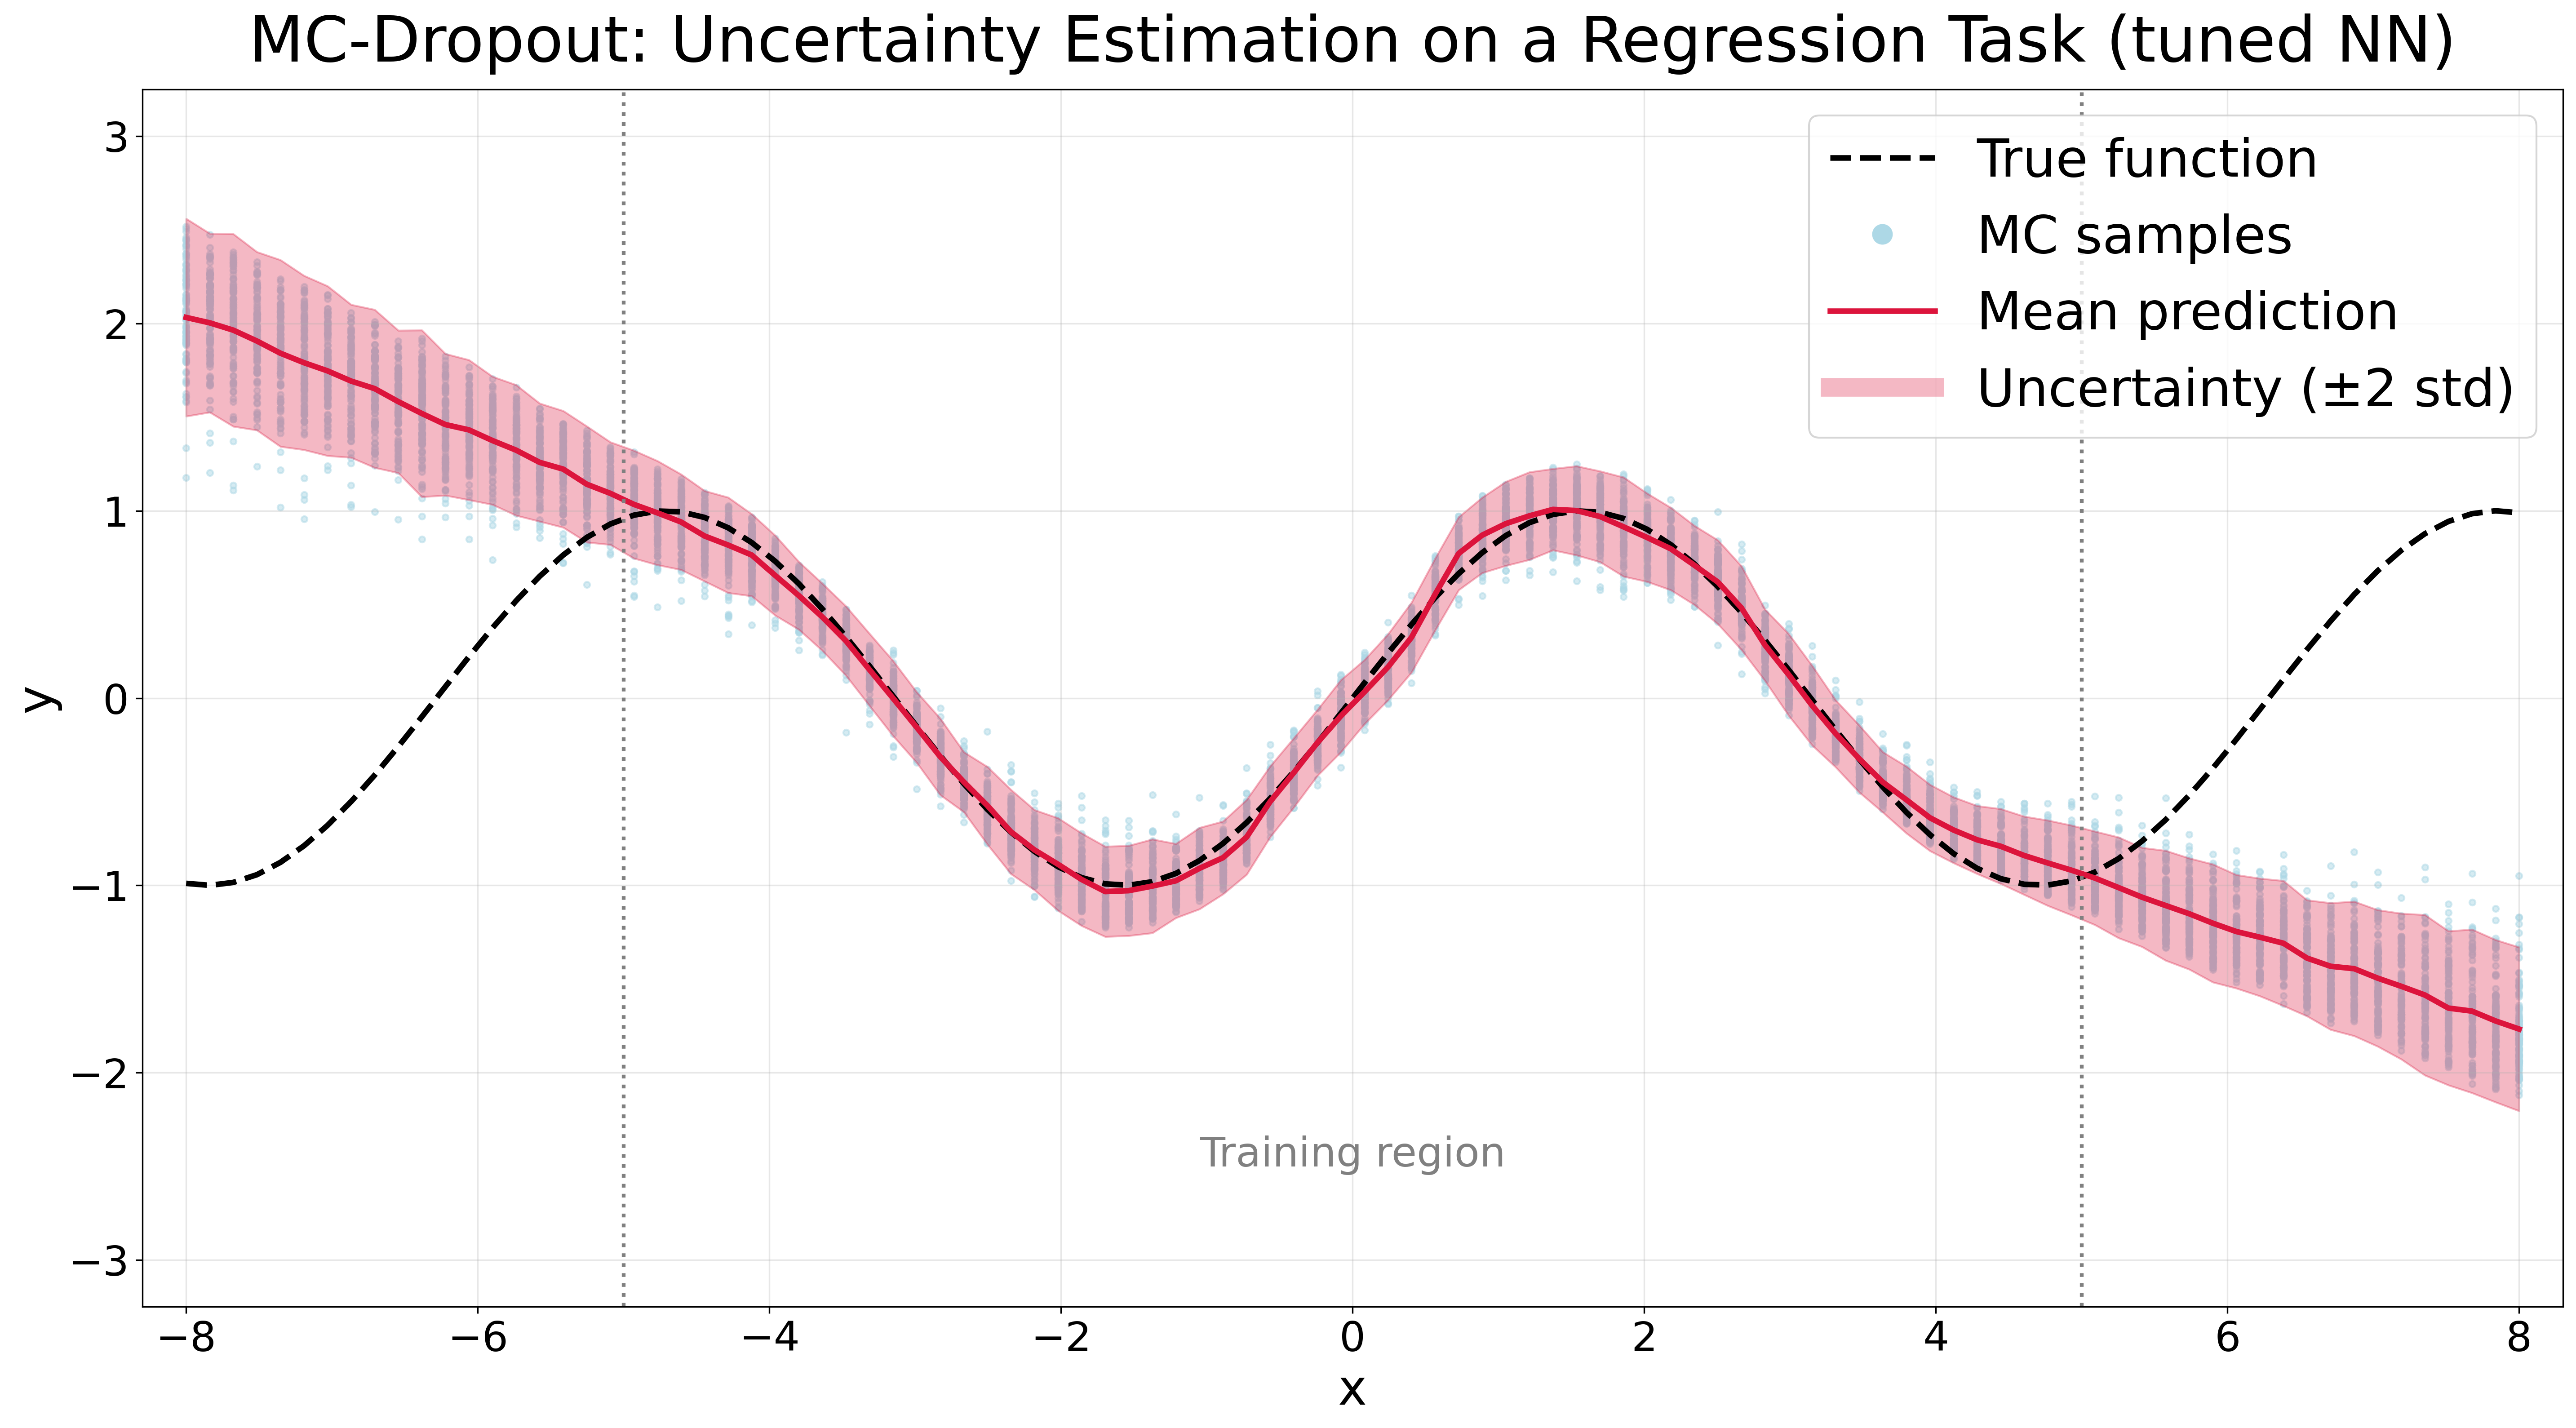
\includegraphics[width=\textwidth]{plots/mcd_reg_tuned.png}
  \end{subfigure}
  
  \vspace{0.3cm}
  \begin{subfigure}{0.8\textwidth}
    \centering
    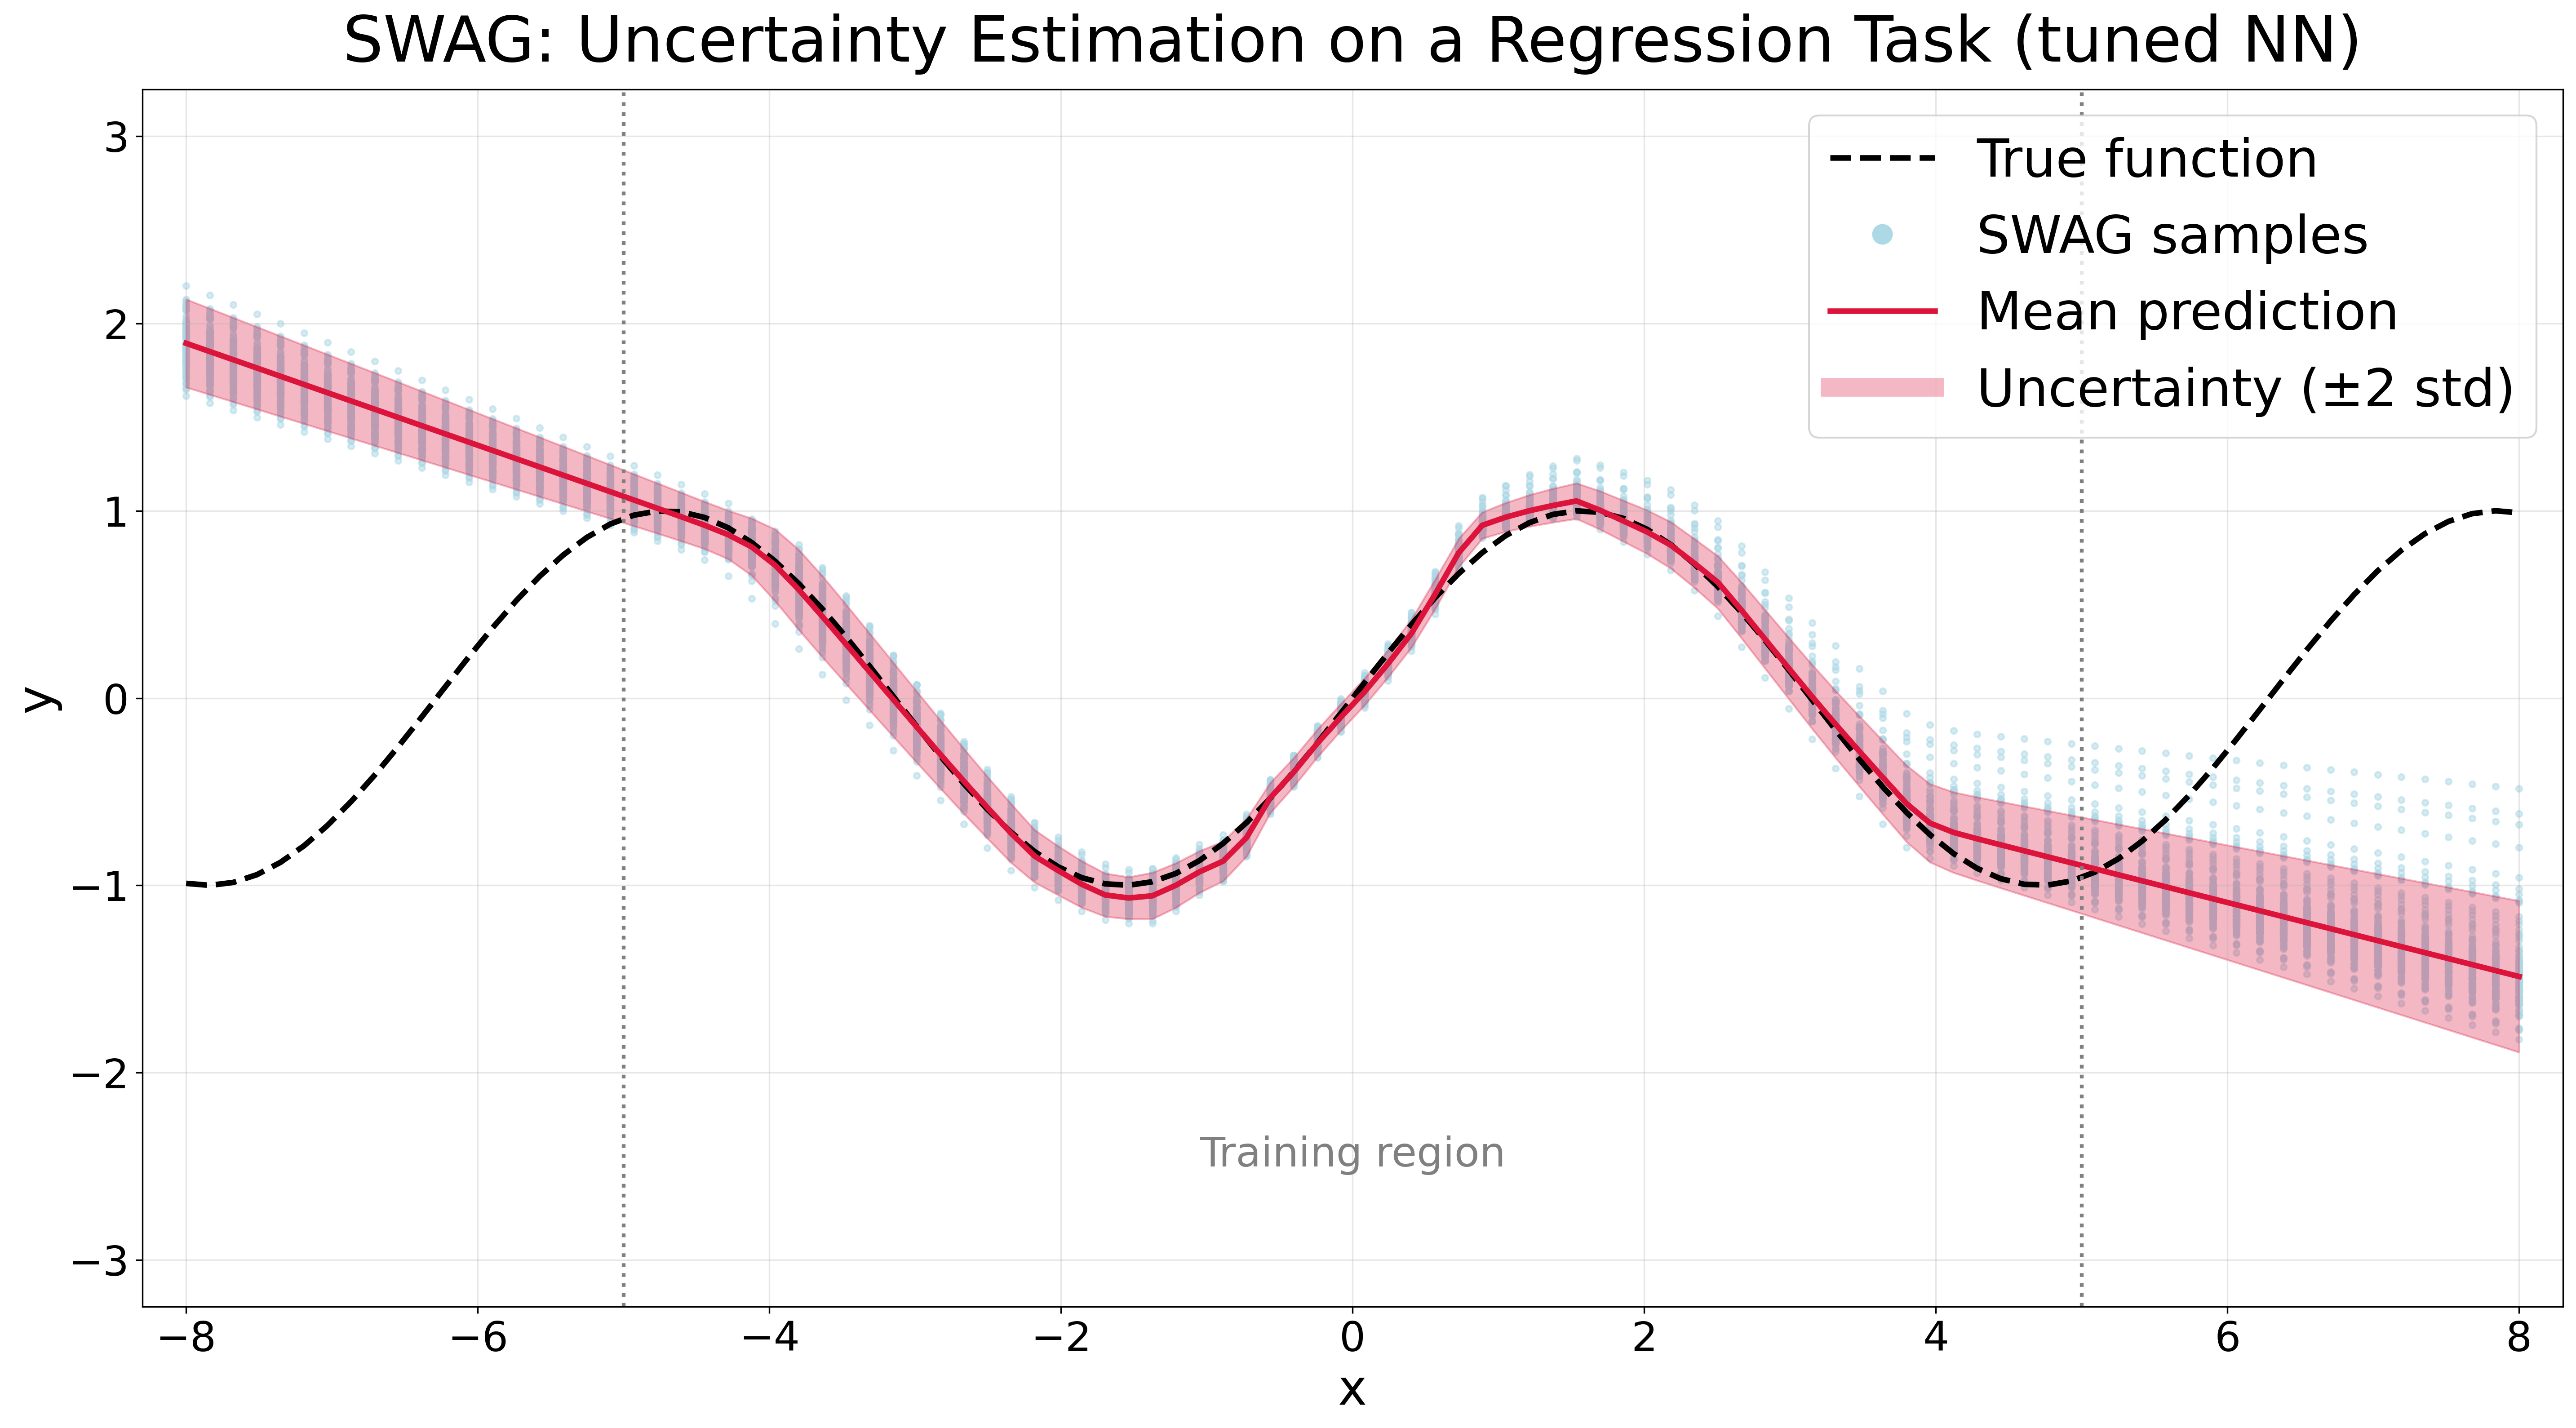
\includegraphics[width=\textwidth]{plots/swag_reg_tuned.png}
  \end{subfigure}
  \caption{Regression uncertainty estimation of a tuned Neural Network: MC-Dropout (top) and SWAG (bottom). Training domain ($|x| \leq 5$) marked by dashed lines.}
  \label{fig:regression_tuned}
\end{figure}

\begin{figure}[ht]
  \centering
  \begin{subfigure}{0.8\textwidth}
    \centering
    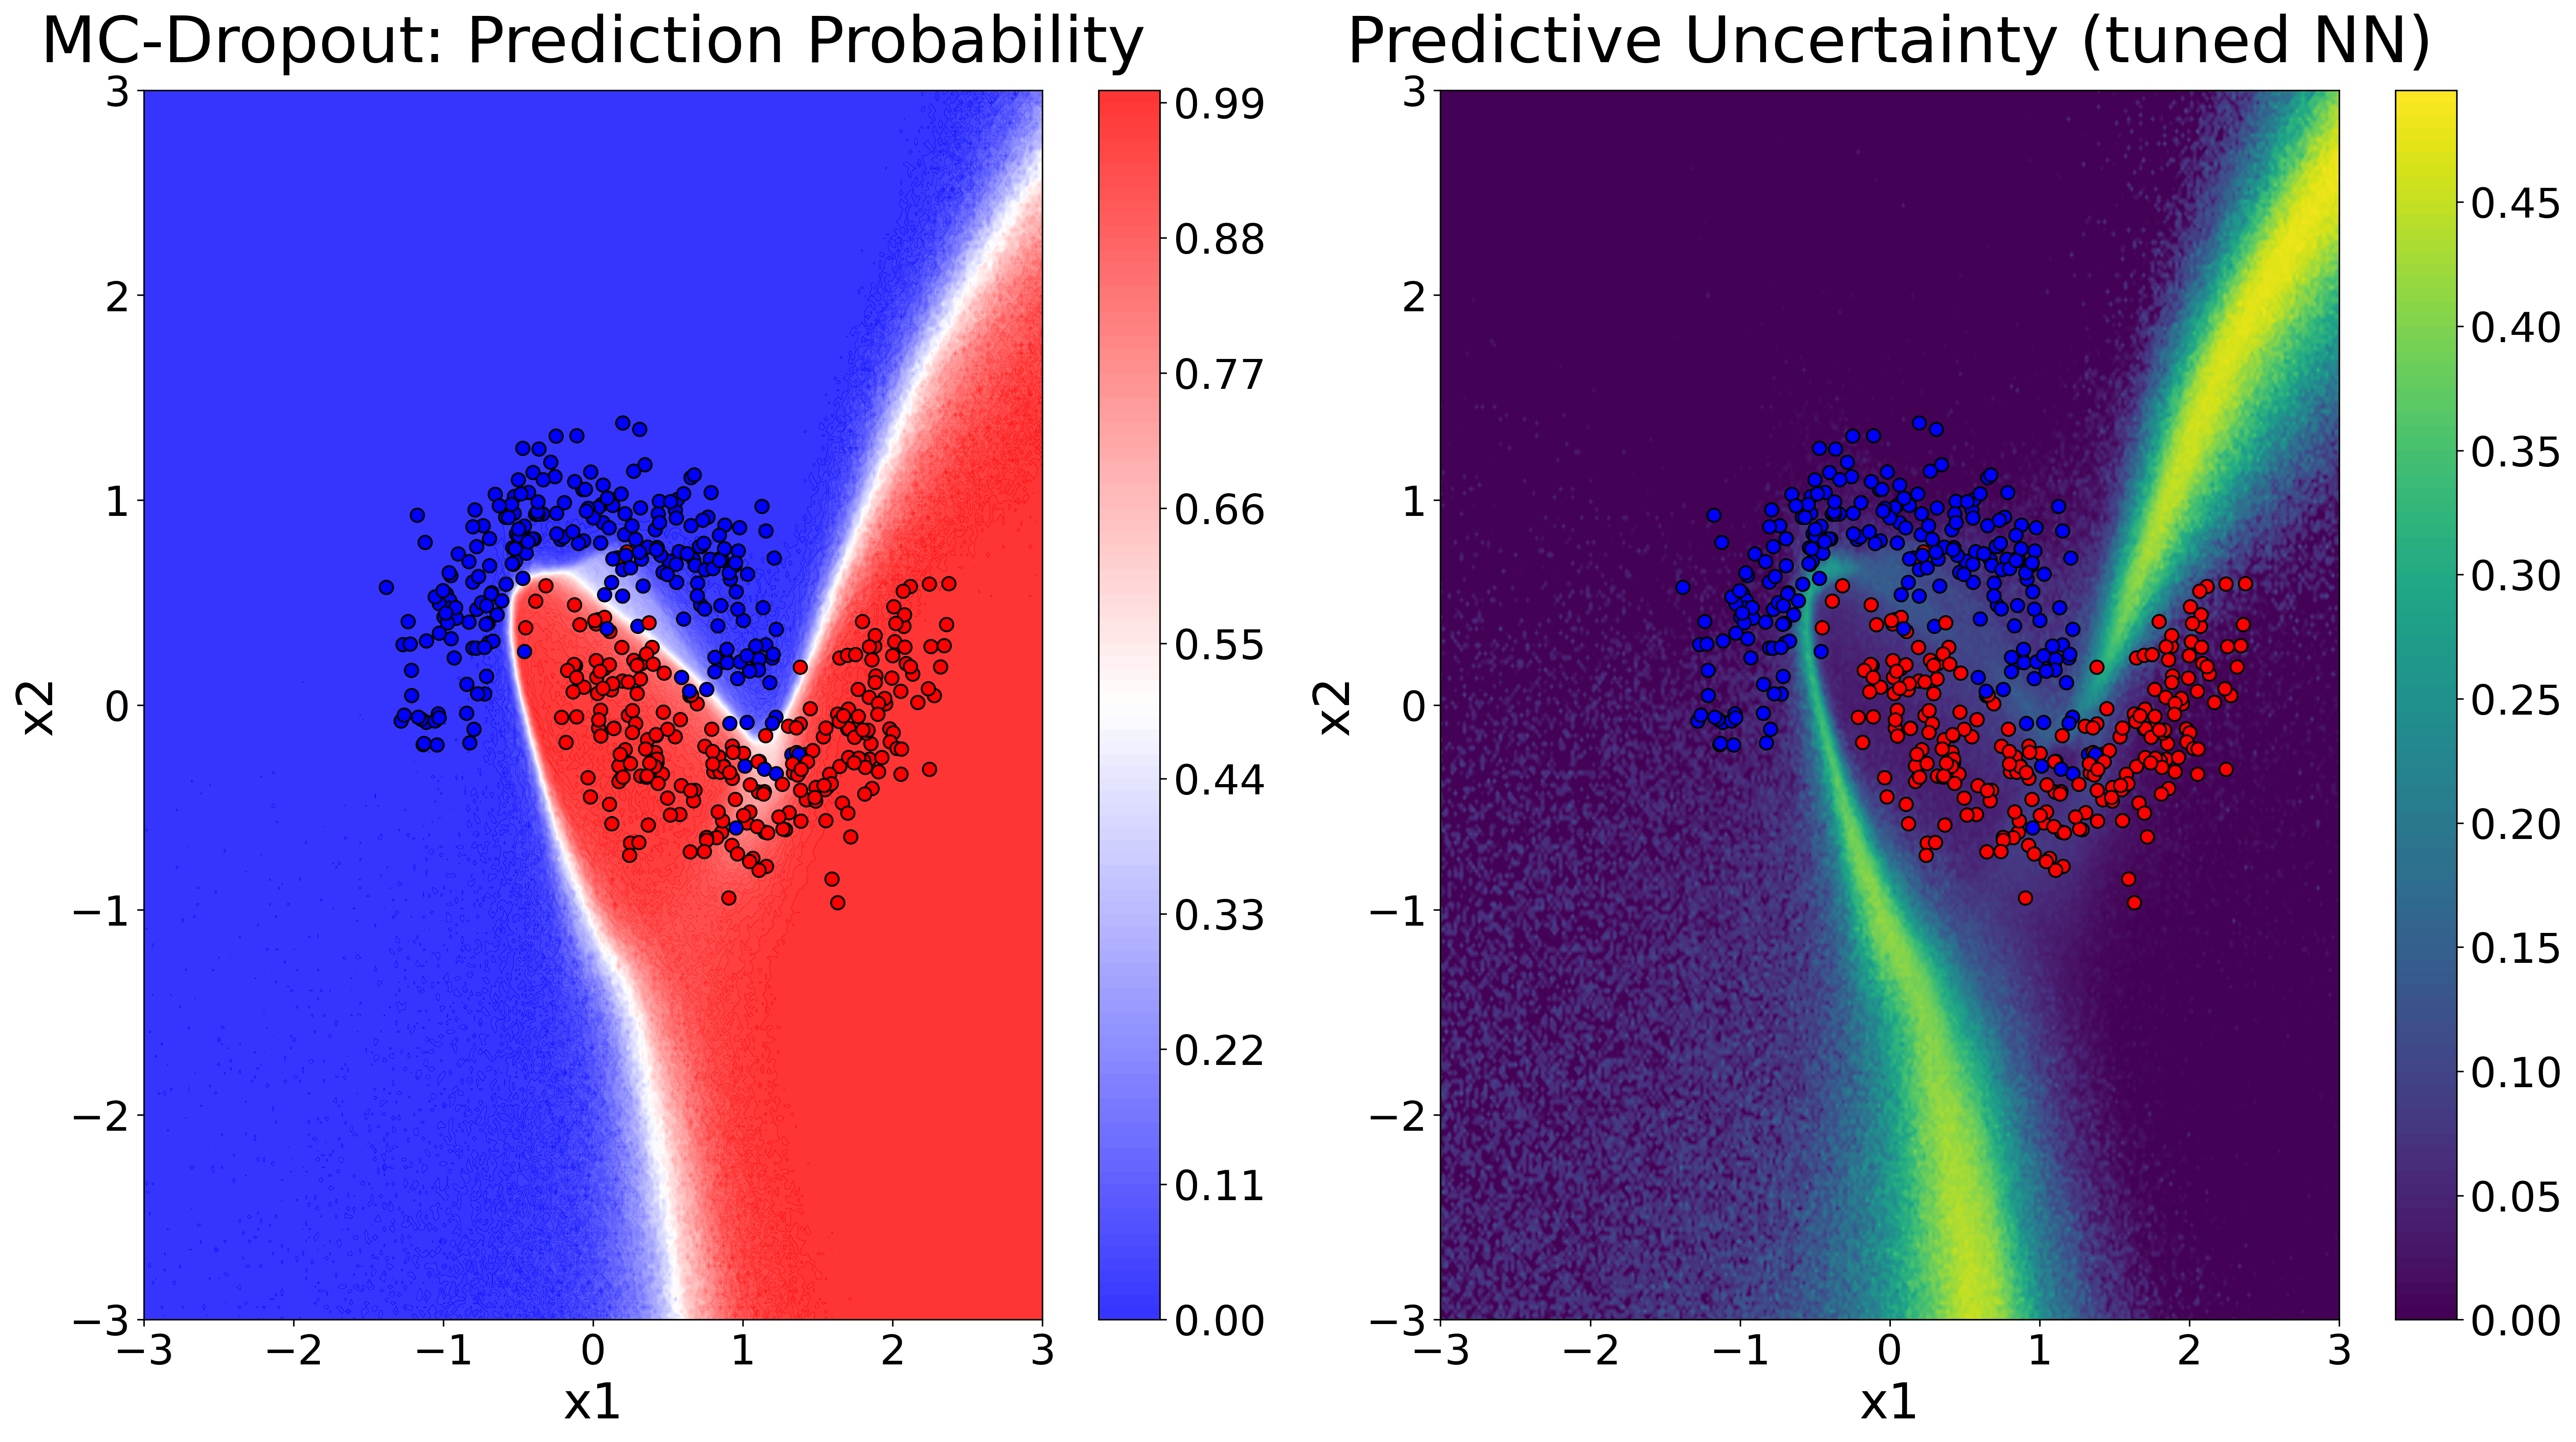
\includegraphics[width=\textwidth]{plots/mcd_cla_tuned.png}
  \end{subfigure}
  
  \vspace{0.3cm}
  \begin{subfigure}{0.8\textwidth}
    \centering
    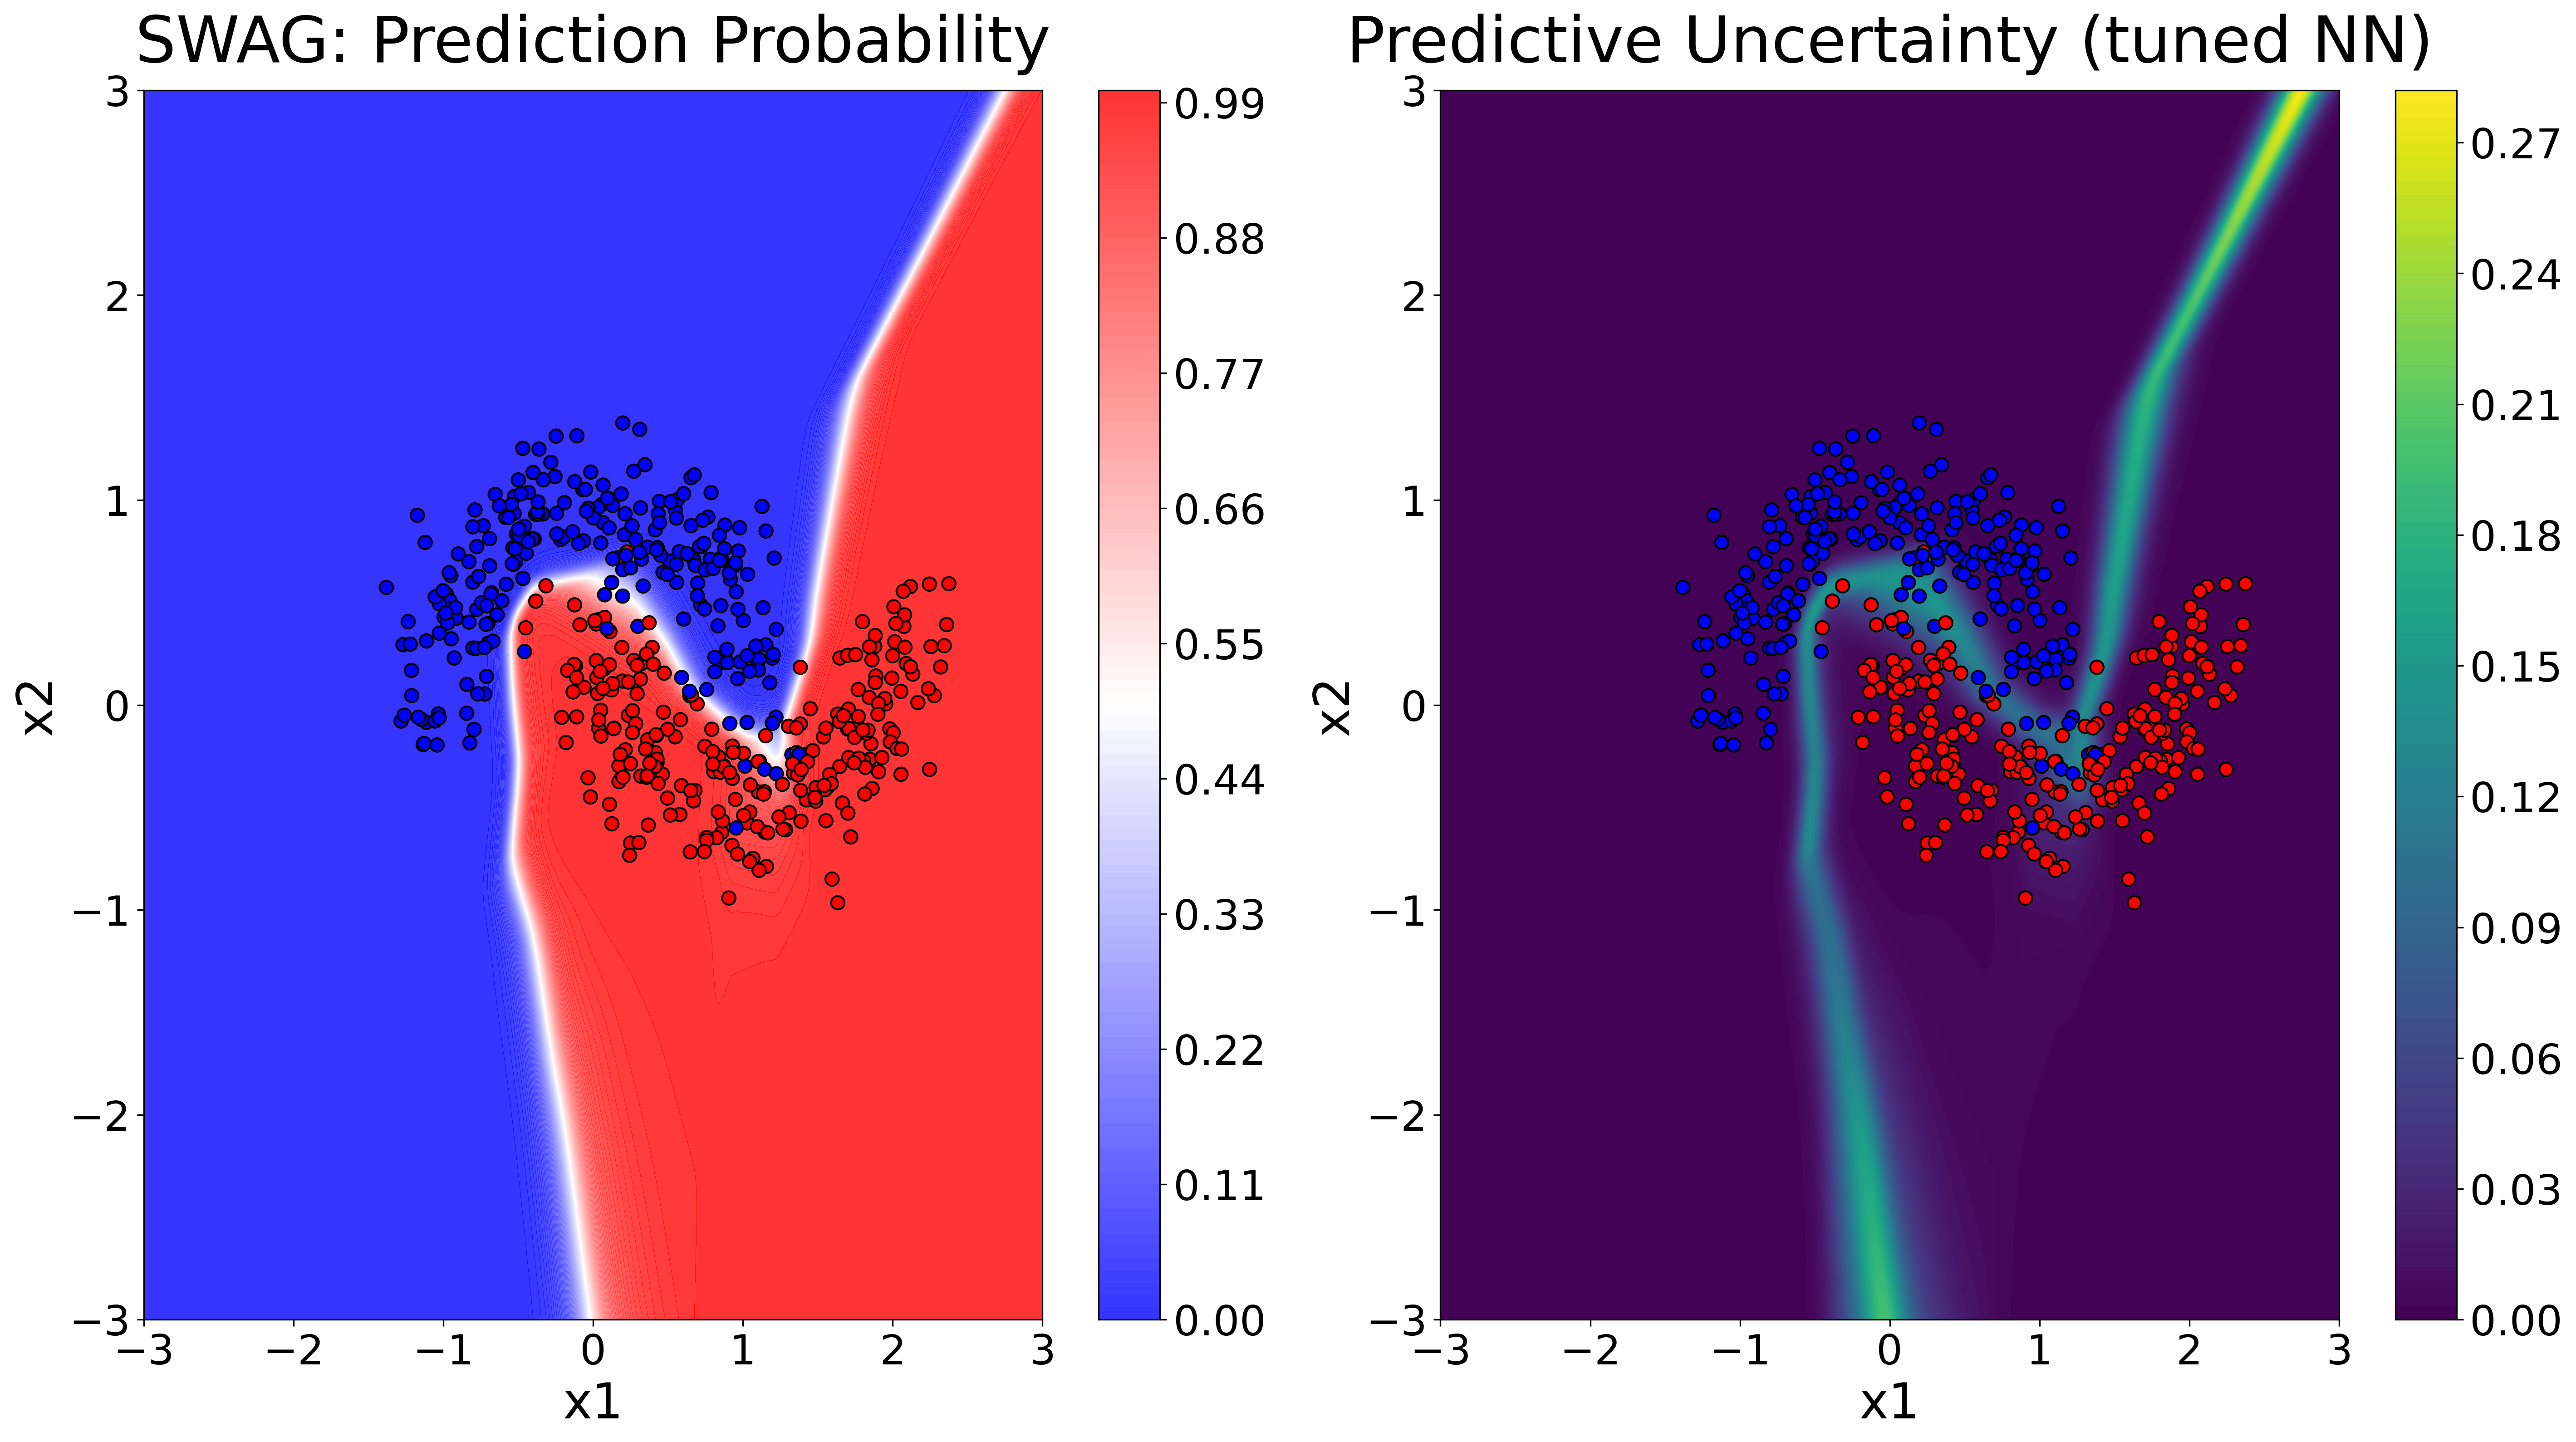
\includegraphics[width=\textwidth]{plots/swag_cla_tuned.png}
  \end{subfigure}
  \caption{Classification uncertainty of a tuned Neural Network: MC-Dropout (top) and SWAG (bottom). Color indicates true class (red/blue).}
  \label{fig:classification_tuned}
\end{figure}

\FloatBarrier

\paragraph{Effect of Dropout Rate on MC-Dropout Uncertainty}
We investigate the sensitivity of MC-Dropout uncertainty estimates to the dropout rate hyperparameter
using the synthetic regression task introduced in Section \ref{exp:synthetic}. While Figure
\ref{fig:regression} presented results with dropout rate = 0.2, we now systematically compare rates of
0.1, 0.3, 0.5 and 0.7. 

As shown in Figure \ref{fig:dropoutrate_comparison}, higher dropout rates produce progressively wider
uncertainty intervals throughout the domain, particularly in extrapolation regions ($|x| > 5$). The mean
prediction also increasingly deviates from the true function as dropout rate increases. These observations
align with findings from \citet{verdoja2021behaviormcdropout}, confirming that dropout rate selection
critically impacts both uncertainty quantification and predictive accuracy.

\FloatBarrier

\begin{figure}[ht]
    \centering
    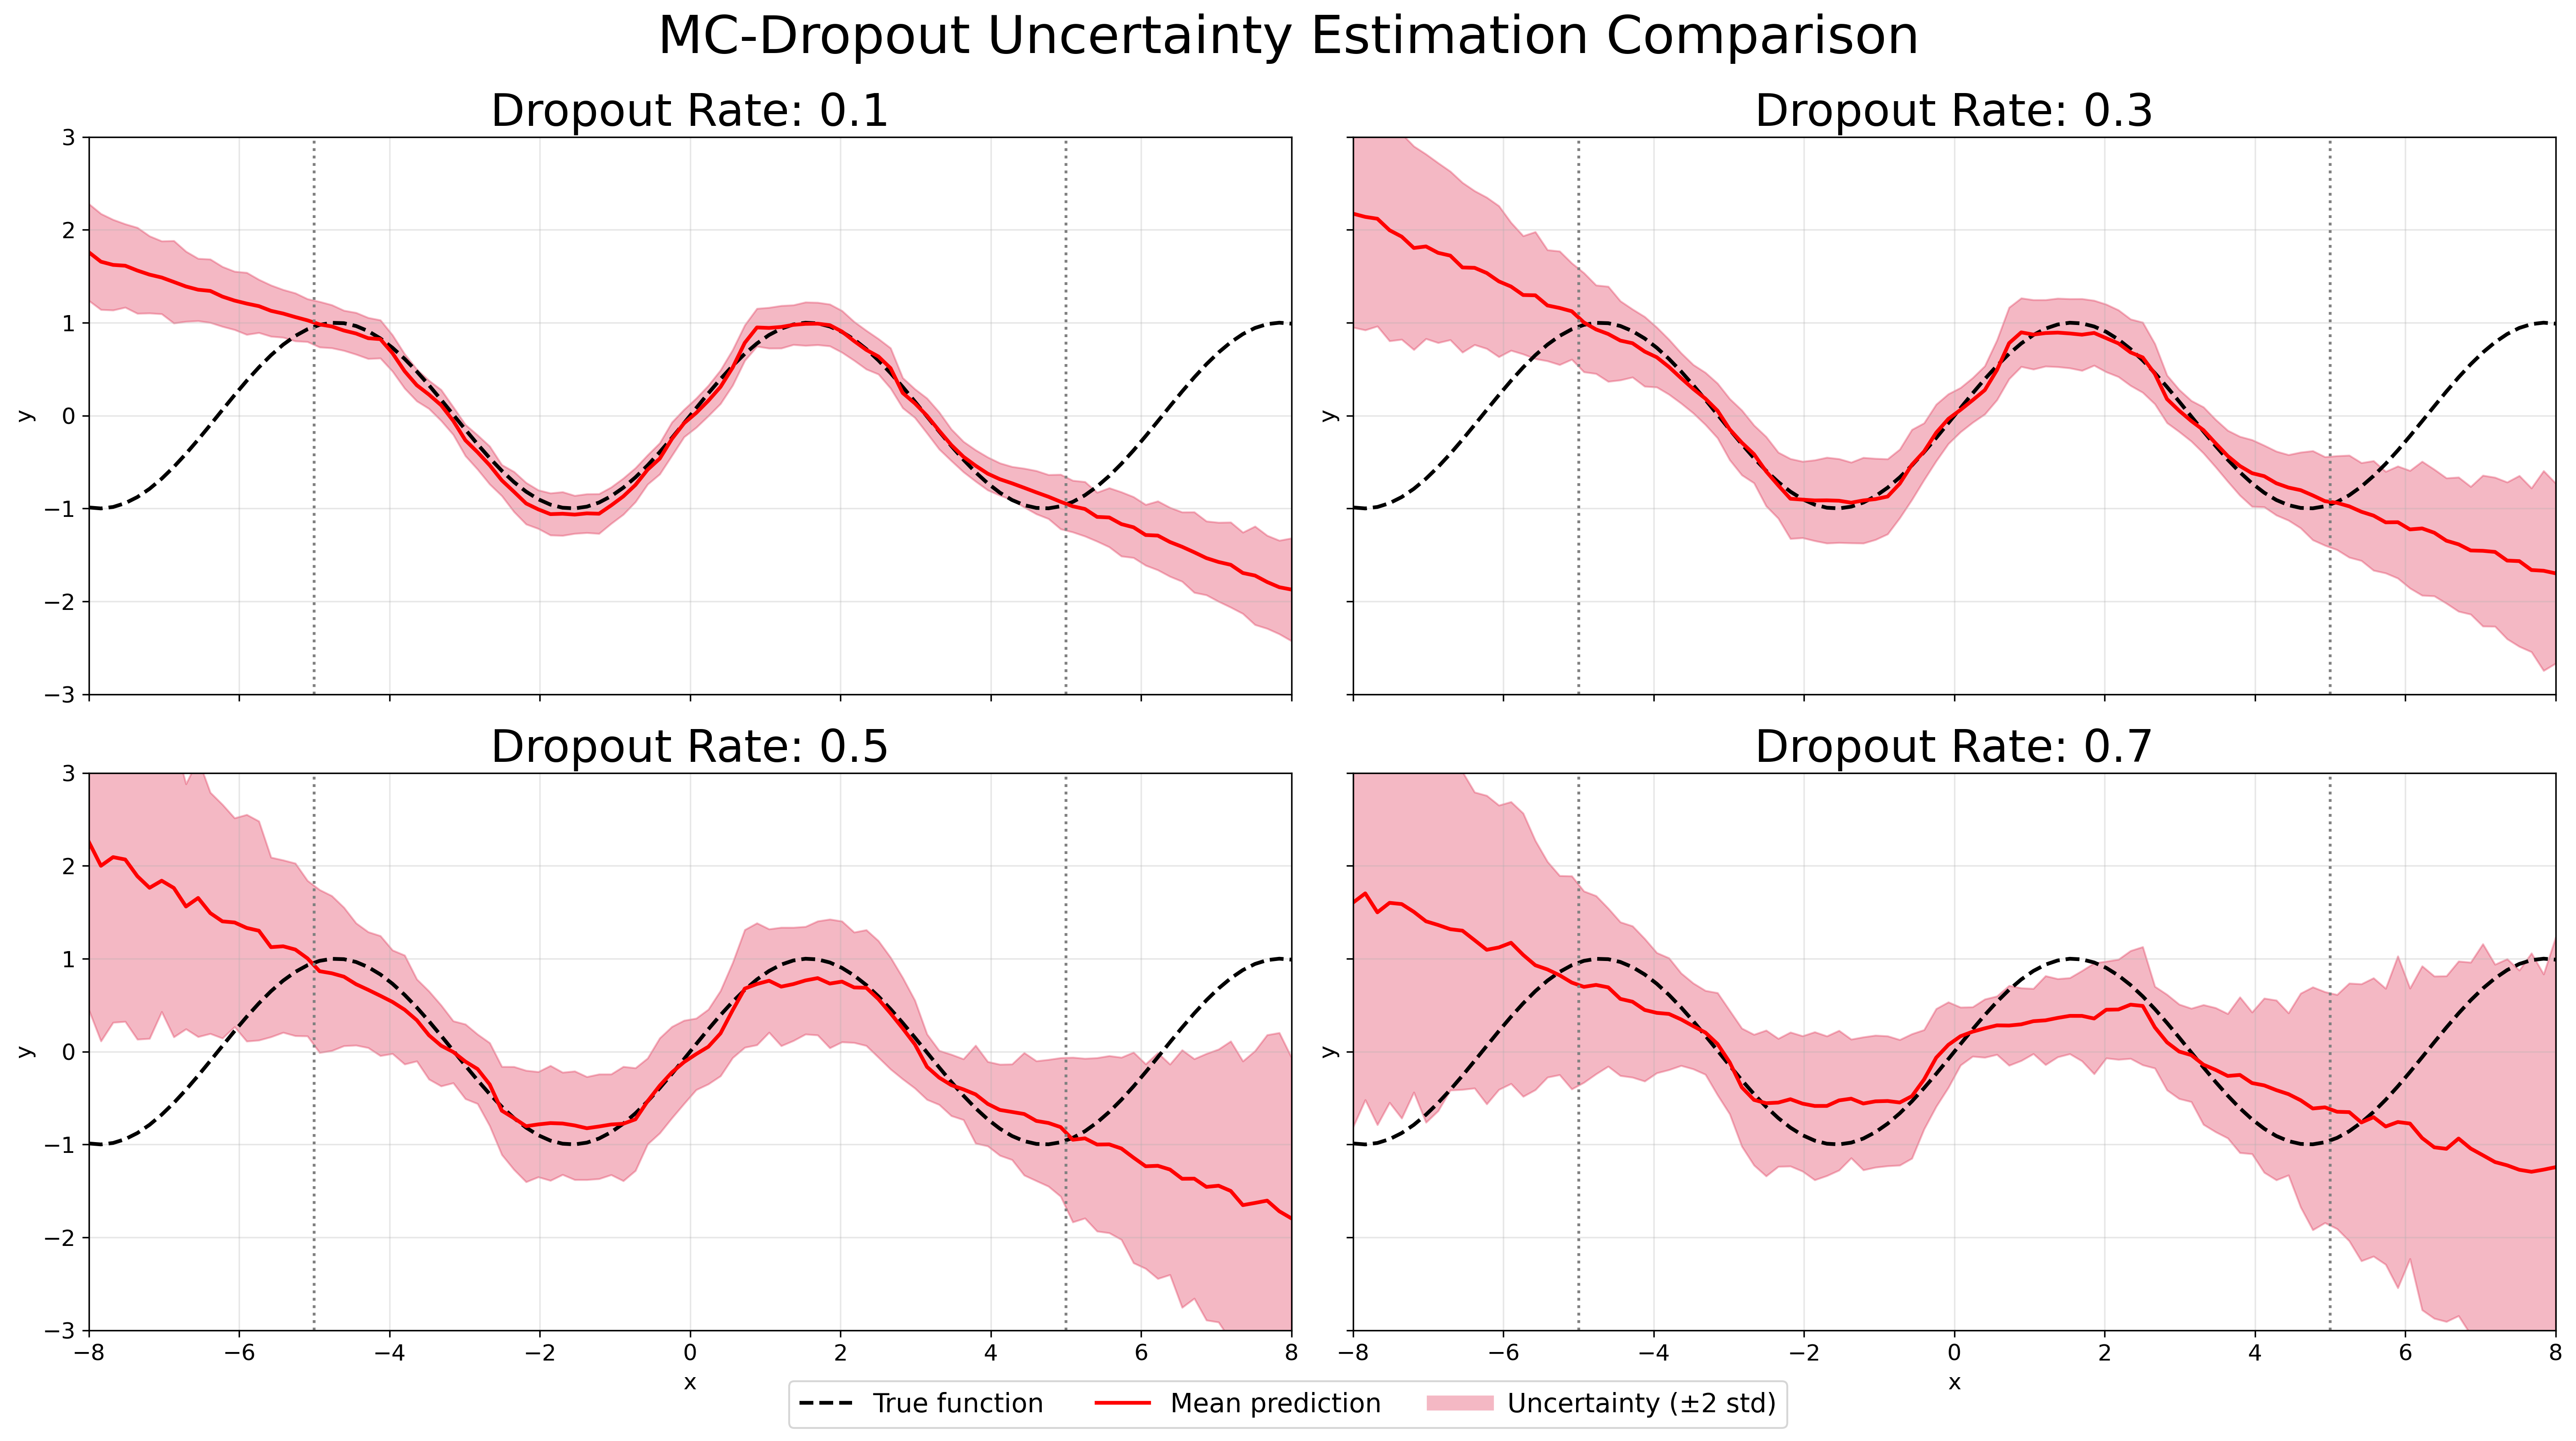
\includegraphics[width=0.9\textwidth]{plots/mcd_reg_comparison_2x2.png}
    \caption{Uncertainty estimation using MC-Dropout with different dropout rates (0.1, 0.3, 0.5, 0.7) on the same regression task.}
    \label{fig:dropoutrate_comparison}
\end{figure}

\FloatBarrier

\paragraph{Predictions with 95\,\% Confidence Intervals on Boston Housing}
Figure \ref{fig:bh_uncertainty_intervals} visualizes predictions against standardized true values with 95\,\% confidence intervals for both methods. The visualization reveals two significant patterns, SWAG exhibits consistently wider confidence intervals (orange bars), particularly pronounced for lower true values in the left side of the plot, confirming its more conservative uncertainty estimation approach. In contrast, MC-Dropout maintains narrower confidence bands that may fail to contain the true values, consistent with its undercoverage tendency. Both methods show generally accurate point predictions closely distributed around the identity line, with only two notable outliers where predictions significantly deviate from true values.

\FloatBarrier

\begin{figure}[ht]
    \centering
    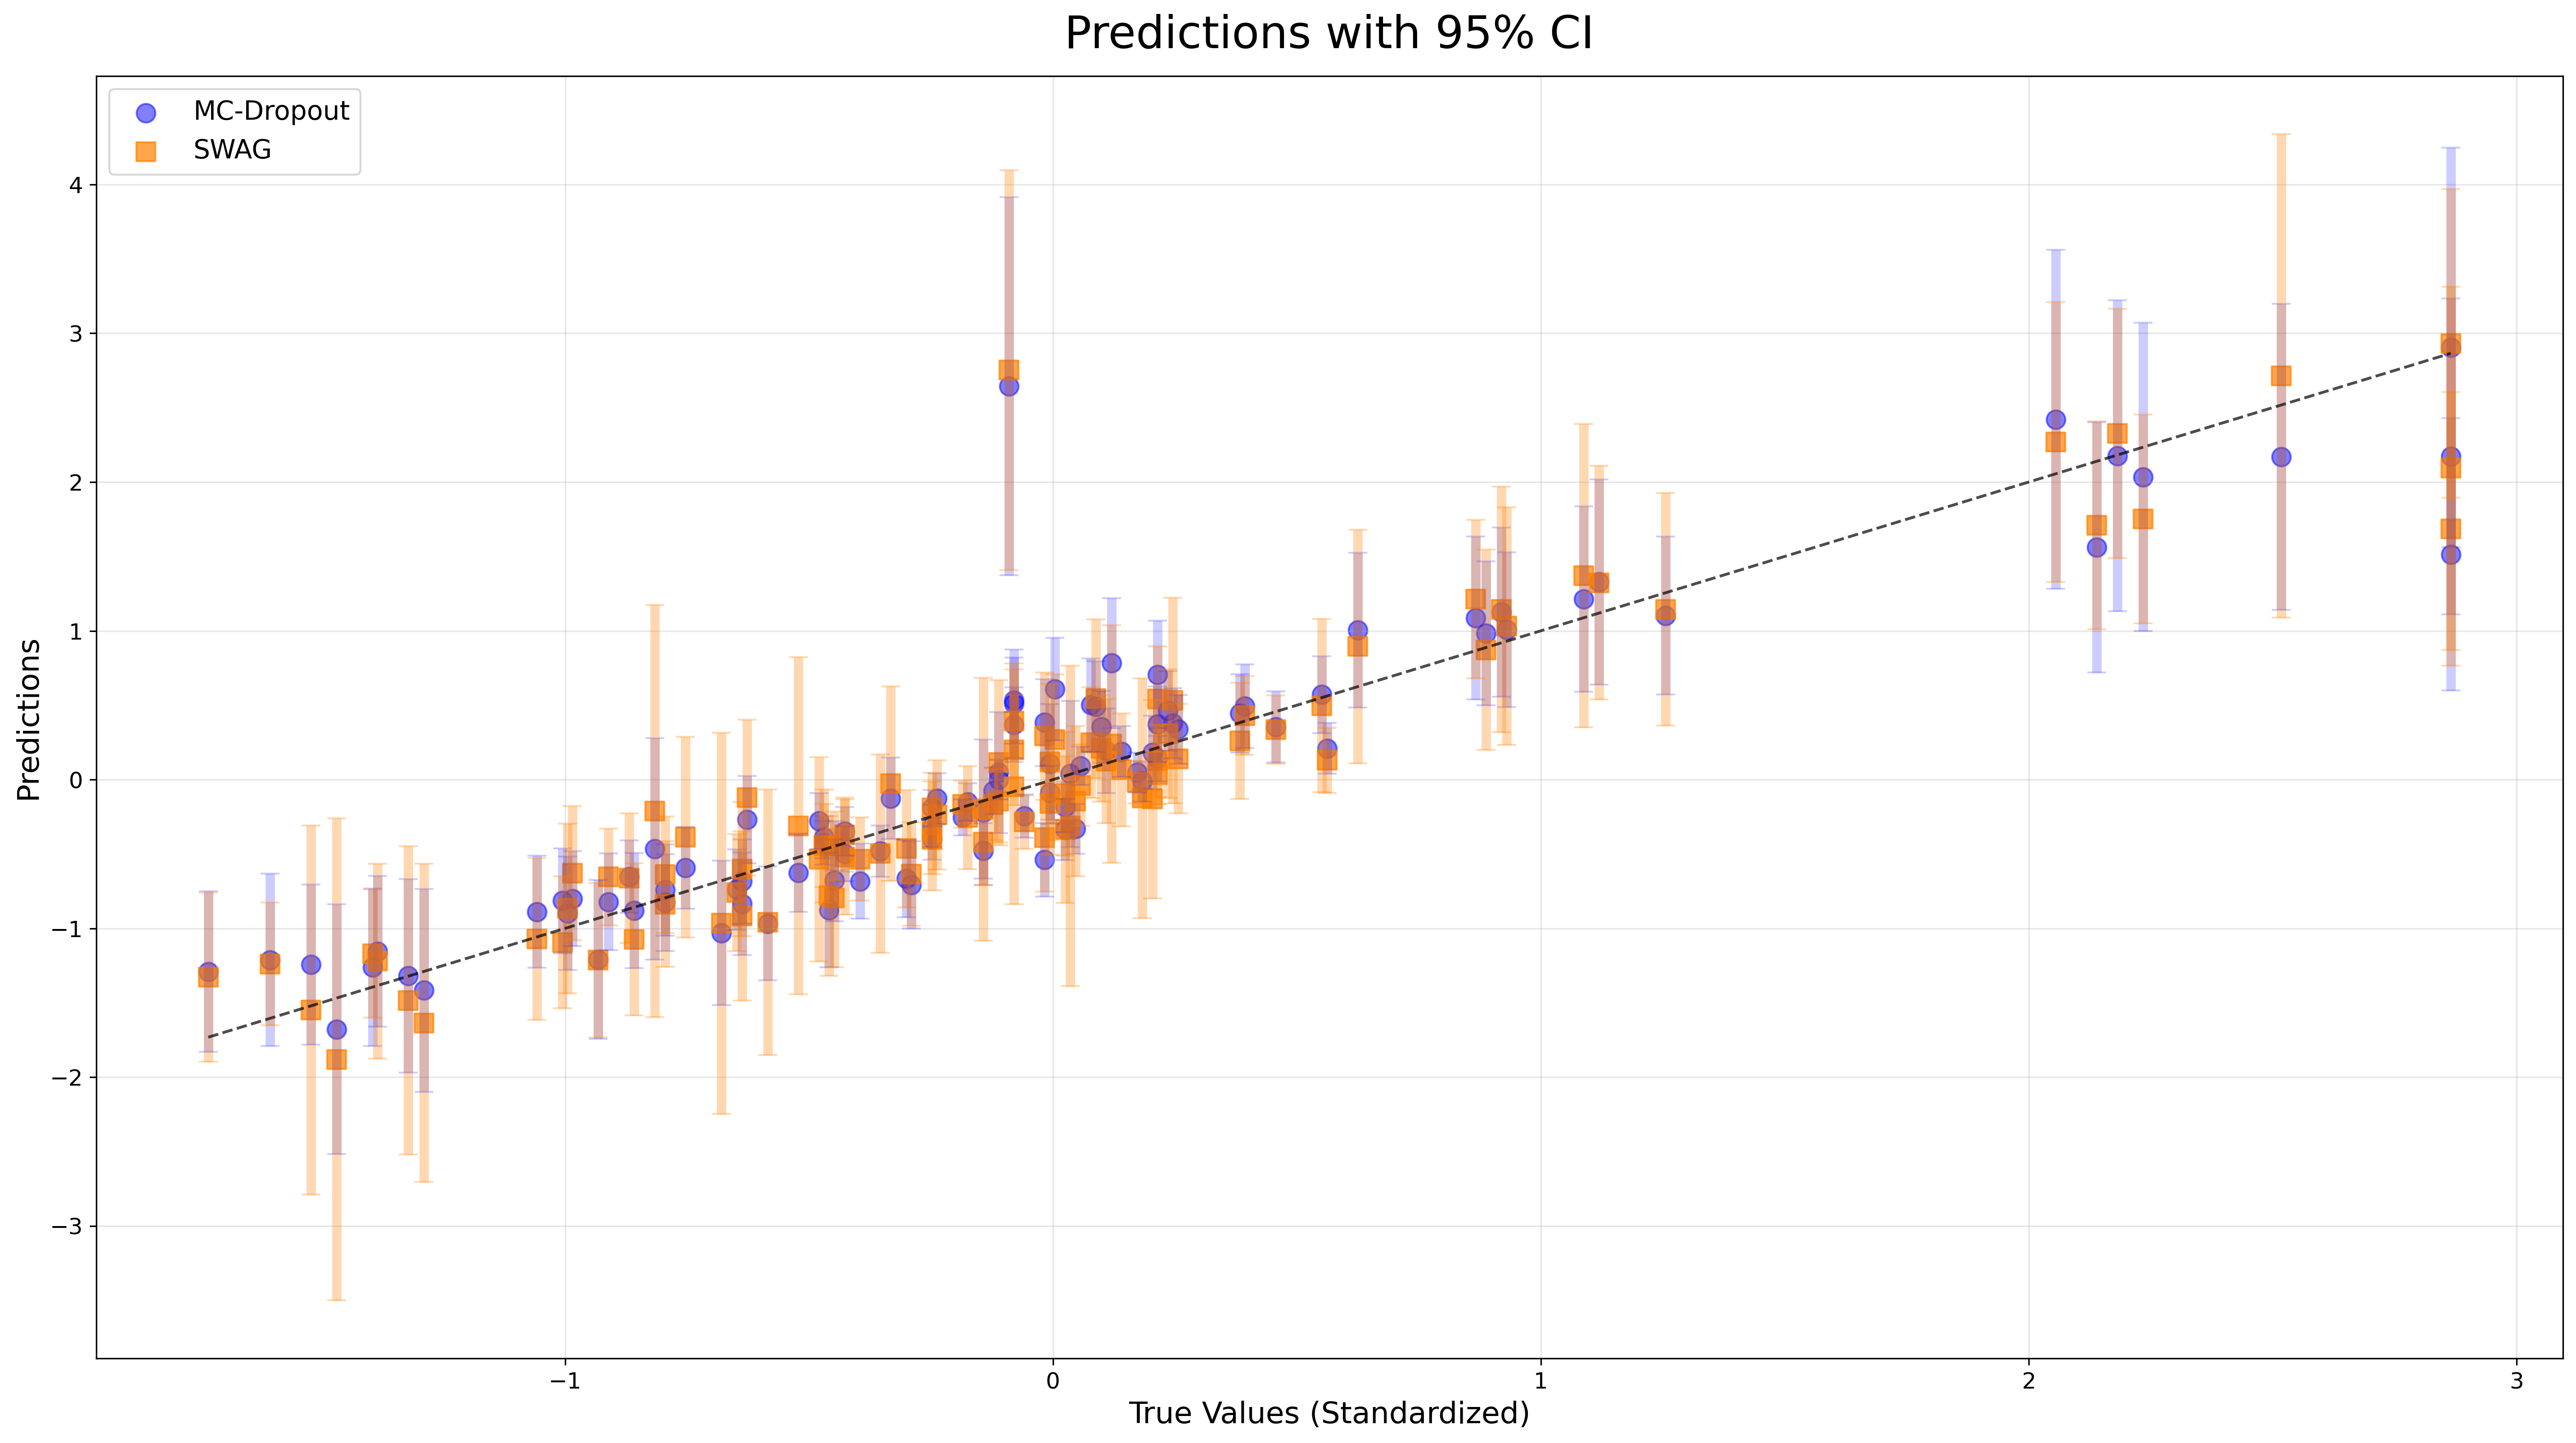
\includegraphics[width=0.9\linewidth]{plots/bh_uncertainty_intervals.png}
    \caption{Predictions with 95\,\% confidence intervals on Boston Housing test set. Dashed line represents perfect predictions (y=x).}
    \label{fig:bh_uncertainty_intervals}
\end{figure}

\FloatBarrier

\paragraph{Residual Analysis on Boston Housing}
Figure \ref{fig:bh_residuals} presents a diagnostic examination of model performance through residual analysis, where residuals represent the difference between observed and predicted values. The visualization reveals randomly distributed points for both MC-Dropout (blue) and SWAG (orange) that symmetrically scatter around the zero-reference line throughout the prediction range. Residual magnitudes demonstrate comparable dispersion for both methods, with no evidence of systematic patterns. This absence of structure indicates a well-calibrated model without significant bias or heteroskedasticity. The random error distribution confirms that both methods capture the underlying relationships in the data effectively, with prediction errors showing no directional tendency.

\FloatBarrier

\begin{figure}[htbp]
    \centering
    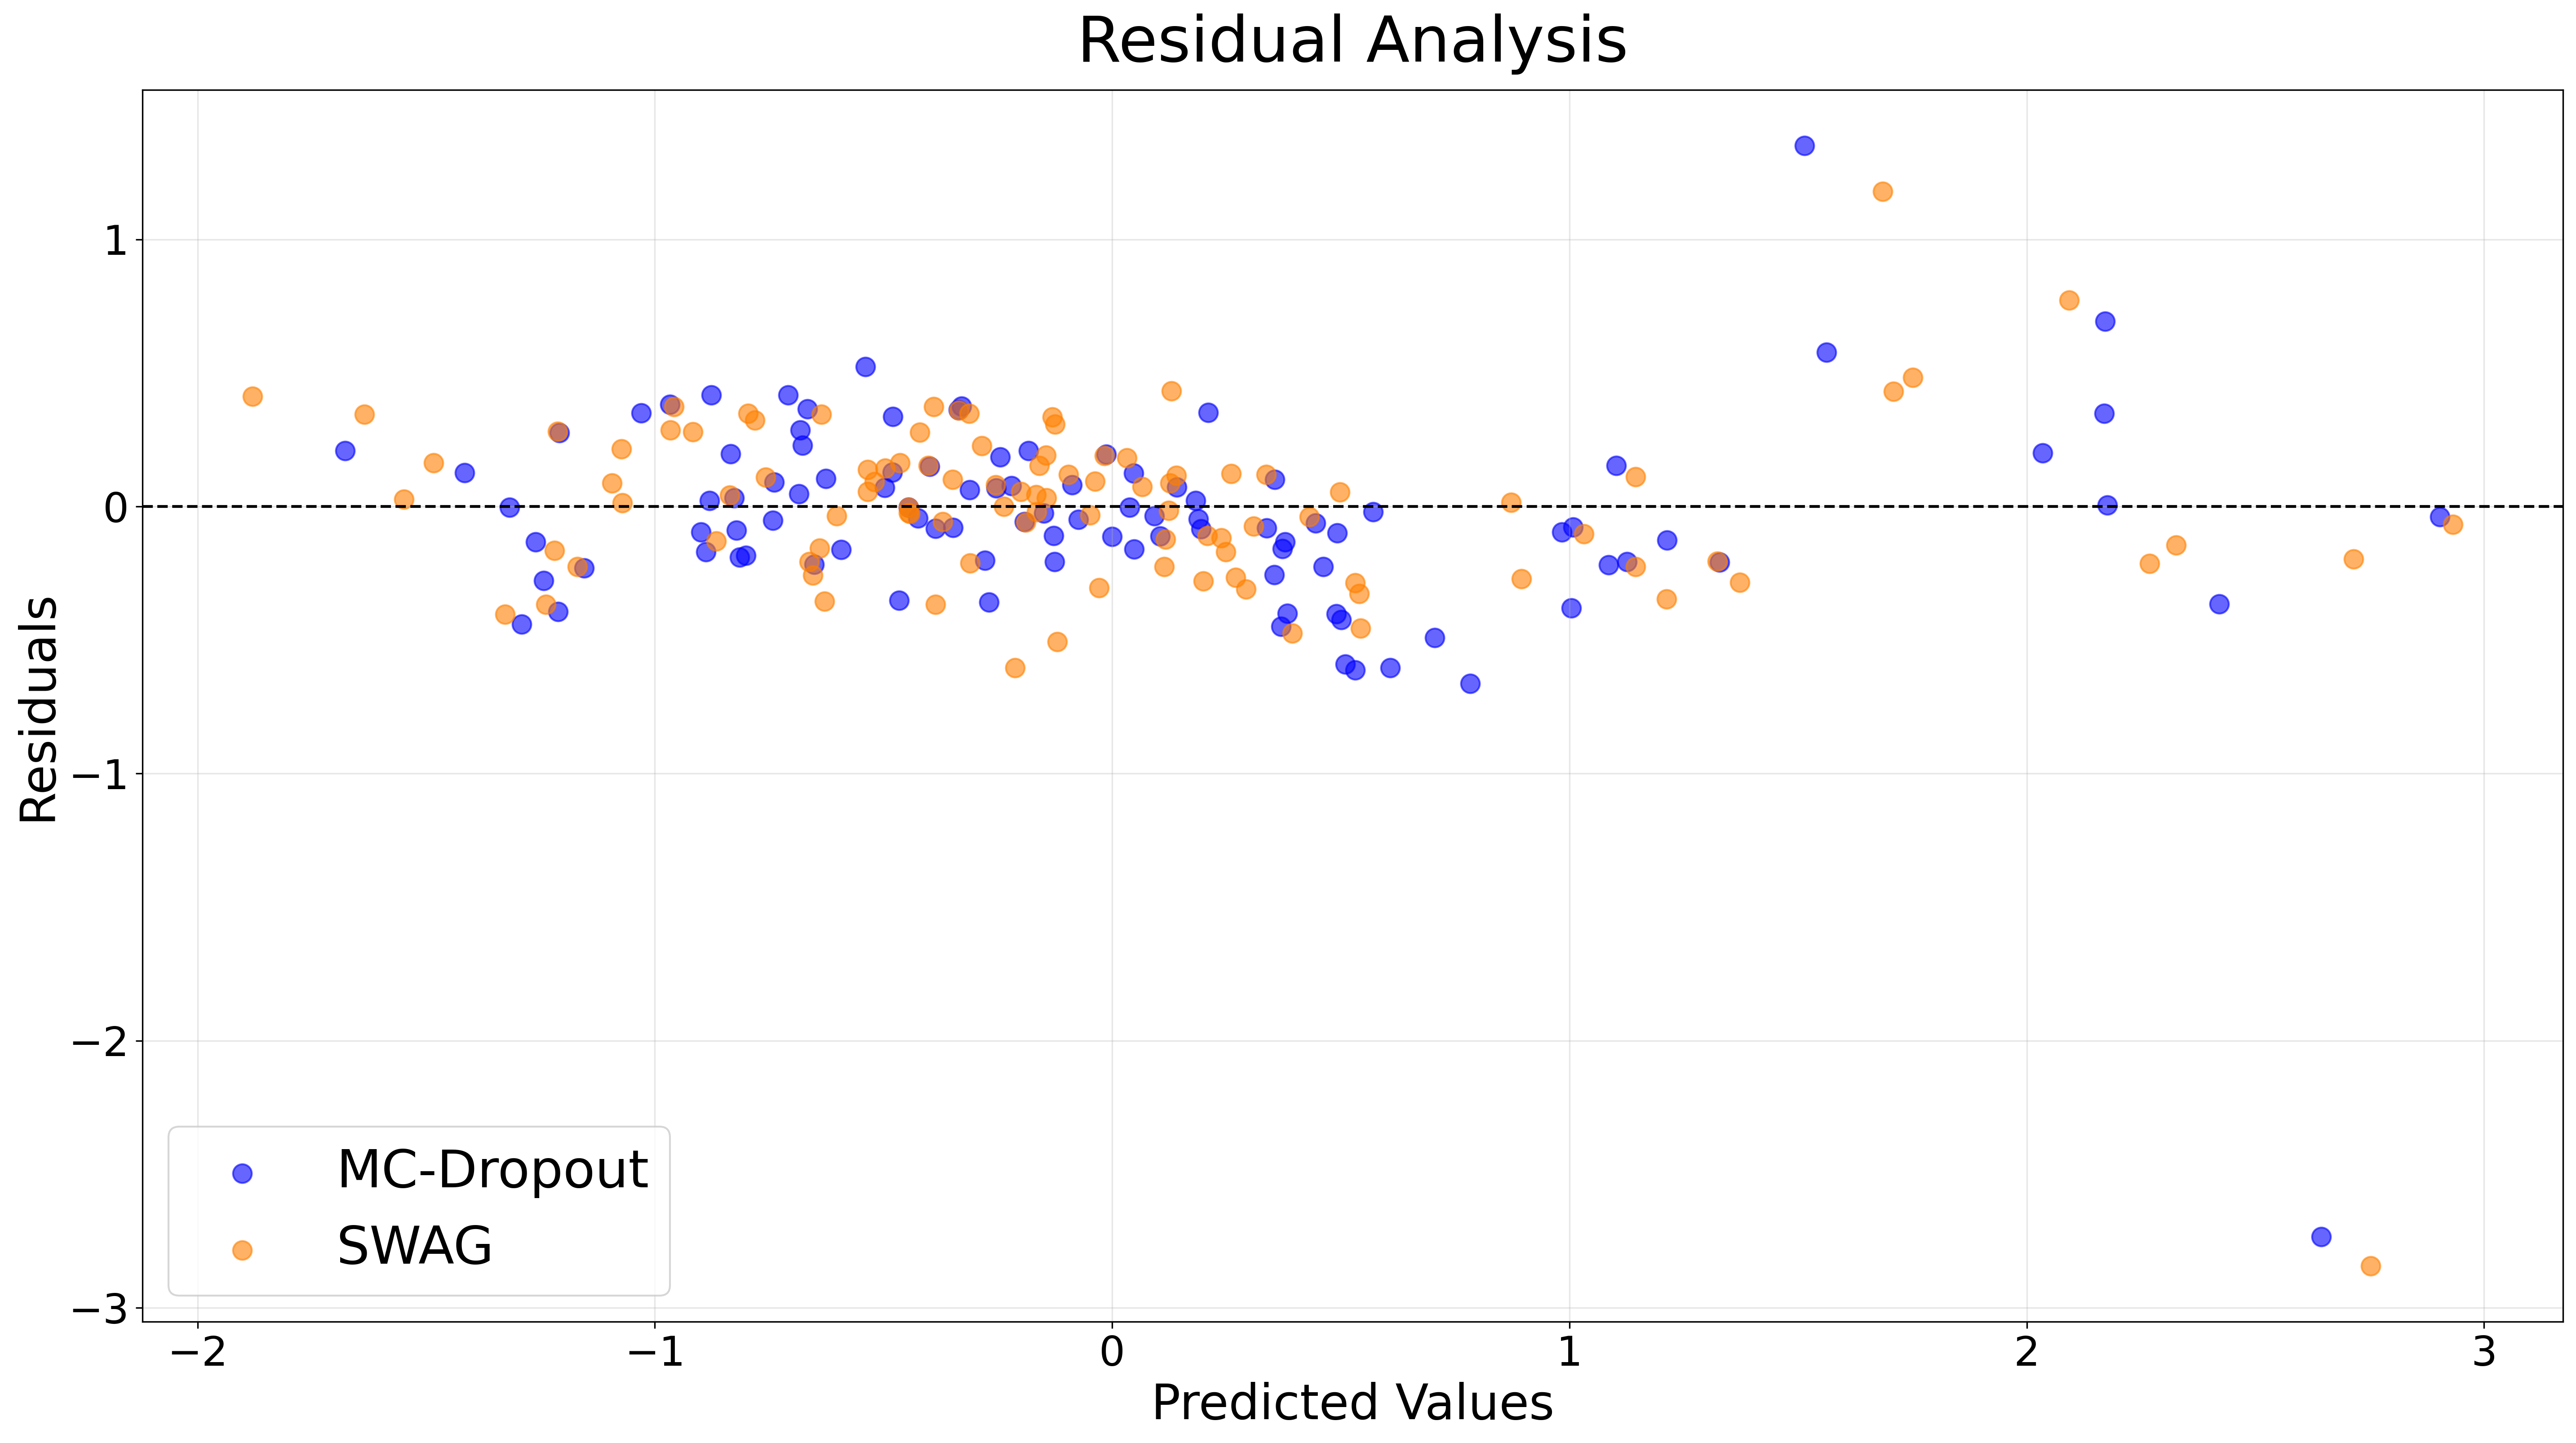
\includegraphics[width=0.9\linewidth]{plots/bh_residuals.png}
    \caption{Residual analysis for Boston Housing predictions. Dashed line represents perfect prediction (residual = 0).}
    \label{fig:bh_residuals}
\end{figure}

\FloatBarrier

\newpage

\section{Electronic appendix}
\label{el_app}

The data, code and figures are available on \url{https://github.com/martin-javier/Seminar_ProbabilisticML}

\newpage
    
% ------------------------------------------------------------------------------
% BIBLIOGRAPHY -----------------------------------------------------------------
% ------------------------------------------------------------------------------

\RaggedRight
\bibliography{bibliography}
\bibliographystyle{dcu}
\newpage

% ------------------------------------------------------------------------------
% DECLARATION OF AUTHORSHIP-----------------------------------------------------
% ------------------------------------------------------------------------------

\Large
\noindent
\textbf{Declaration of authorship} 
\vspace{0.5cm}
\noindent
\normalsize

I hereby declare that the report submitted is my own unaided work. All direct 
or indirect sources used are acknowledged as references. I am aware that the 
Thesis in digital form can be examined for the use of unauthorized aid and in 
order to determine whether the report as a whole or parts incorporated in it may 
be deemed as plagiarism. For the comparison of my work with existing sources I 
agree that it shall be entered in a database where it shall also remain after 
examination, to enable comparison with future Theses submitted. Further rights 
of reproduction and usage, however, are not granted here. This paper was not 
previously presented to another examination board and has not been published.
\\

\vspace{1cm}
\textcolor{orange}{Location, date} \\

\vspace{3cm}

\noindent\rule{0.5\textwidth}{0.4pt} \\

\textcolor{orange}{Name}

% ------------------------------------------------------------------------------

\end{document}
